\PassOptionsToPackage{unicode=true}{hyperref} % options for packages loaded elsewhere
\PassOptionsToPackage{hyphens}{url}
%
\documentclass[]{article}
\usepackage{lmodern}
\usepackage{amssymb,amsmath}
\usepackage{ifxetex,ifluatex}
\usepackage{fixltx2e} % provides \textsubscript
\ifnum 0\ifxetex 1\fi\ifluatex 1\fi=0 % if pdftex
  \usepackage[T1]{fontenc}
  \usepackage[utf8]{inputenc}
  \usepackage{textcomp} % provides euro and other symbols
\else % if luatex or xelatex
  \usepackage{unicode-math}
  \defaultfontfeatures{Ligatures=TeX,Scale=MatchLowercase}
\fi
% use upquote if available, for straight quotes in verbatim environments
\IfFileExists{upquote.sty}{\usepackage{upquote}}{}
% use microtype if available
\IfFileExists{microtype.sty}{%
\usepackage[]{microtype}
\UseMicrotypeSet[protrusion]{basicmath} % disable protrusion for tt fonts
}{}
\IfFileExists{parskip.sty}{%
\usepackage{parskip}
}{% else
\setlength{\parindent}{0pt}
\setlength{\parskip}{6pt plus 2pt minus 1pt}
}
\usepackage{hyperref}
\hypersetup{
            pdftitle={AIMEE Milestone 7 Report: Weird Mario},
            pdfauthor={Peli Grietzer},
            pdfborder={0 0 0},
            breaklinks=true}
\urlstyle{same}  % don't use monospace font for urls
\usepackage{graphicx,grffile}
\makeatletter
\def\maxwidth{\ifdim\Gin@nat@width>\linewidth\linewidth\else\Gin@nat@width\fi}
\def\maxheight{\ifdim\Gin@nat@height>\textheight\textheight\else\Gin@nat@height\fi}
\makeatother
% Scale images if necessary, so that they will not overflow the page
% margins by default, and it is still possible to overwrite the defaults
% using explicit options in \includegraphics[width, height, ...]{}
\setkeys{Gin}{width=\maxwidth,height=\maxheight,keepaspectratio}
\setlength{\emergencystretch}{3em}  % prevent overfull lines
\providecommand{\tightlist}{%
  \setlength{\itemsep}{0pt}\setlength{\parskip}{0pt}}
\setcounter{secnumdepth}{0}
% Redefines (sub)paragraphs to behave more like sections
\ifx\paragraph\undefined\else
\let\oldparagraph\paragraph
\renewcommand{\paragraph}[1]{\oldparagraph{#1}\mbox{}}
\fi
\ifx\subparagraph\undefined\else
\let\oldsubparagraph\subparagraph
\renewcommand{\subparagraph}[1]{\oldsubparagraph{#1}\mbox{}}
\fi

% set default figure placement to htbp
\makeatletter
\def\fps@figure{htbp}
\makeatother


\title{AIMEE Milestone 7 Report: Weird Mario}
\author{Peli Grietzer}
\date{April 6, 2021}

\begin{document}
\maketitle

\hypertarget{executive-summary}{%
\section{Executive Summary}\label{executive-summary}}

Until now our contributions to AIMEE focused on using genetic
programming as a way to find a variety of interesting states. States
arising from a system on which a small amount of data and the execution
flow could be controlled by an attacker but no new instructions could be
added.

During this stage of the project we have explored the possibility to
generalize and apply some of the lessons learned until now to other
systems in weird states. In particular, we have explored the possibility
of using a technique known as deep reinforcement learning, to train
neural network agents able to find ``interesting'' results by sending
inputs to a video game which is on a weird state. This weird state
allows playing the game under relatively normal conditions until a
specific item is acquired which further modifies the program state. In
this second weird state, the behaviour of the game varies widely and may
even allow the system to execute code derived from the player's actions.
Reinforcement learning was deemed appropriate for this approach because
it can adapt to the changes in state that different inputs to the game
may produce over time.

Reinforcement learning is based on rewards. Therefore, we considered
three main basic approaches: rewarding when a specific game counter
increased; rewarding when the computer program counter had unseen
instructions; and rewarding increases on the maximum brightness of the
screen.

The research found that such rewards successfully incentivize the agents
to trigger execution of weird-states, since weird states can produce
significantly higher rewards than normal use of the game. The research
additionally found that trained agents can implicitly distinguish
triggers for profitable weird-state execution from triggers for
unprofitable weird-state execution, demonstrating the trained agent's
ability to statistically predict properties of emergent execution.
Finally, the research also produced a negative result: it was found that
although mean score scaled with training and rose further for more
powerful, compute-intensive agent types, these factors don't improve an
agent's chance to earn extreme high scores. This may be a result of the
agent prioritizing mid-gain lower risk strategies over huge-gain and
high risk ones. A second and related cause may be the inability of
reinforcement-learning agents to continue searching for new strategies
after discovering a reliable strategy.

In general, it was found that reinforcement learning is promising for
researching statistical patterns in emergent-execution spaces, but may
be less promising as a direct technique for `proof by demonstration'
exploitation studies. The negative part of the conclusion remains
tentative, since resource limitations ruled out experimenting with
industrial-scale deep reinforcement learning, and deep reinforcement
learning is known to be sensitive to scale.

Future work will aim to integrate deep reinforcement learning and our
genetic programming techniques. The literature suggests that hybrid
reinforcement/genetic techniques are well-suited for conditions where
pure reinforcement learning prematurely settles on a mediocre strategy.
The current iteration of our genetic programming framework Berbalang was
designed for easy integration with deep-learning systems, so we expect
the integration process to be rapid.

\hypertarget{overview}{%
\section{Overview}\label{overview}}

The purpose of our AIMEE Weird Mario project is to use ML techniques to
study regularities in emergent execution in a setting where the user's
input primitives are far from the natural level of abstraction of the
program's control flow.

We use the emulated SNES video-game environment as a logistically
efficient proxy to the case exploiting complex applications by means of
highly constrained user input---constrained, in this case, to a small
alphabet of control signals: up, down, right, left, A, B, X, Y, select,
left-pad, right-pad. Working within an emulated video-games environment
has two crucial advantages:

First, there is a strong foundation of existing open source
infrastructure for interfacing ML algorithms with an emulated SNES
environment, as well as well-developed best-practices regarding the
appropriate learning algorithms, network architectures, and
hyperparameters for deep reinforcement learning in arcade environments.

Second, exploitation of emulated SNES games is an active and
well-documented area of amature `straw hat' exploitation research. The
exploitation terrain of the SNES game Super Mario World, in particular,
has been extensively albeit non-systematically studied and documented by
speed-runners, modders, and recreational hackers.

When programming a weird machine by `playing' a video game, one
generally cannot hope for stable semantics at the level of input
subsequences. E.g. the semantics of input subsequences is unlikely to be
stable under permutation of the order of subsequences. Instead, one
might hope to demonstrate that an ML algorithm can learn general (for
the given weird machine) strategies for context-dependent action. In a
way such that the algorithm implicitly applies equivalent or related
abstract program-manipulations using different input-sequences in
different circumstances.

The ideal demonstration of a learnable general (for the given weird
machine) strategy would be training an agent to discover very long
chains of distinct weird states. This is because in order to maintain
compositionality when acting in a previously unseen weird state the
agent must apply previously learned principles to a novel situation.
Learning to maintain compositionality requires powerful generalization
that applies not only `horizontally', across weird states encountered in
different training runs, but `vertically', from weird states that are
accessible in early training runs that produce only short chains to
weird states that appear only in longer chains and therefore do not
appear often during early training.

A weaker demonstration of a learnable general (for the given weird
machine) strategy relies on adding stochasticity to the operation of the
weird machine, such that the algorithm cannot simply memorize effective
sequences. This is the approach traditionally used in reinforcement
learning research when the learning environment is deterministic: the
added stochasticity ensures that performance improvement as measured by
increase of mean reward over the course of training reflects
generalization.

\hypertarget{introduction-super-mario-world-exploitation}{%
\section{Introduction: Super Mario World
Exploitation}\label{introduction-super-mario-world-exploitation}}

Super Mario World followed on the dynamics of prior Super Mario games
while introducing new dynamics such as the ability to play with a
companion called Yoshi or additional power-ups like the `feather cape'.
The game was significantly more complex than the original Mario Bros
game, and features an early example of `world-driven' video-game design,
which resulted in a significant number of issues and glitches. As usual,
most of these glitches have effects ranging from full game crashes to
minor visual artifacts. Some of these glitches can be combined to
trigger interesting side effects, including the ability to execute code
introduced manually by the player.

The way in which these glitches operate differs significantly from the
ROP scenarios that we studied in phase 1 of AIMEE, wherein the
artificial intelligence (AI) had significant control over the state of
the system. On the one hand, in the ROP scenarios the AI had free reign
over a relatively large share of the system's memory, and was restricted
only by a prohibition on executing new code. On the other, in the Weird
Mario project the AI's on point of control over the system is the
ability to enter inputs using a ``virtual'' controller emulating the
original SNES game controller (which can be seen below). Additionally,
while on our first iteration the status of the system's memory was known
and maintained during the whole execution of the attack, in these
experiments the environment spontaneously varies over time in ways that
are chaotically conditioned by the agent's actions, making the memory
states unpredictable and therefore requiring more complex techniques.

\begin{figure}
\centering
\includegraphics{./img/113896374-297a4900-97ca-11eb-8b9a-9ef456c05e3c.png}
\caption{Super Nintendo Entertainment System controller}
\end{figure}

In the following subsections, we review the concepts necessary to
understand some of the glitches used and their impact on emergent
execution.

\hypertarget{power-up-states}{%
\subsection{Power-up states}\label{power-up-states}}

In Super Mario World, the character controlled by the player can acquire
a set of items that change the game mechanics slightly. Such items are
known as power-ups because the mechanic changes benefit the player in
some way. The game keeps track of the current state of the character
using a number known as the power-up state. This number is used by the
system in a variety of ways, including deciding what to do once a new
power-up is acquired.

In the game, when the player acquires a power-up, instead of applying a
lot of complex if/else logic conditions to decide what to do, the game
chooses a table based on the number defining the current character state
and then uses that table to get an address that points to some code that
(when executed) carries out the desired actions. This is significantly
faster and more elegant than having a large number of conditions. The
problem with this approach, however, is that if for some reason the
number used to decide which item to retrieve is larger than the number
of items on the table, the code will instead interpret whatever data is
placed on memory after the table as the item to be retrieved.

Under normal conditions, the game itself ensures that the player's
power-up state, the number indicating the game-dynamics to follow, is
never larger than the tables indexed making such strange behavior
imposible. Despite that, if a player can somehow increase that number
over the number of known states, the player can then make the game
retrieve content from a location in the system's memory that was not
originally intended to be used as an address for code-execution, and
then run code from that address.

\hypertarget{power-up-incrementation}{%
\subsection{Power-up incrementation}\label{power-up-incrementation}}

Power-up incrementation is the name given to different techniques that
allow the player to increase the power-up state beyond 4 (which is the
maximum number the game intended to allow). The techniques used to
trigger this vary and exploit different weird behaviours that trigger
under very specific corner cases. These techniques can and have been
applied manually by certain players and are behind most of the glitch
exploitation allowing interesting effects like directly jumping to the
game ending or loading and executing a new game using code entered by
the player using the controller.

Over time, faster and more reliable approaches to attain these
objectives have been found and, currently, it is possible to achieve
such a behavior already on the first level of the game.

\hypertarget{creamsicle-mario}{%
\subsection{Creamsicle Mario}\label{creamsicle-mario}}

From the states that can be reached using the techniques mentioned
above, of particular interest are the cases when this number is 6 or 22
since when acquiring certain power-ups, they allow executing code from
areas that can be influenced through the player actions. With power-up
state 6 the item is the 1-up mushroom which is very rare since it
normally grants the player an extra life. With power-up state 22 there
are several such items, including the item known as the `standard'
power-up mushroom -- a very common item that makes the character grow in
size among other things. Unlike 1-up mushrooms, standard mushrooms can
be saved for later use by the player under certain circumstances.

This last power-up state (power-up state 22) is also known as
``Creamsicle Mario'' because of the orangeish color the character
acquires, and is kept across levels as long as the character does not
enter in contact with any hazard or enemy. This state is also fairly
stable and contained under other conditions, allowing playing the game
as you normally would.

\hypertarget{open-bus-access}{%
\subsection{Open bus access}\label{open-bus-access}}

Once the power-up triggering this behaviour is acquired in the
Creamsicle Mario state, what's known to SNES hackers as an `open bus'
anomaly takes place. To understand what this anomaly does, we have to
first understand the basics of how a processor works.

Processors have different components that perform different operations
on the data they contain, to allow for greater flexibility and reduce
costs all these components are usually interconnected using a data bus.
A data bus can be seen as something similar to the air connecting
different employees in an office. When an employee wants to send a
message to a colleague he can just shout the message into the air so
that it will reach its destination. On the process, all other employees
will also hear the information but ignore it. On a processor, the data
is instead placed on a set of wires that connects all of the components
handling data together so that it reaches the intended destination. In
order for the right component to then process and handle the data,
additional internal signals are added so that: only one of the
components will put data on the wires at a time; and only the desired
components read the data from the wires. With the appropriate
coordination all of these components act in an ordered manner performing
the intended modifications on data given by a set of instructions.

But, what happens when nobody writes into the data bus and somebody
reads from it? The behaviour varies from processor to processor but on
the original processor used by the SNES, the cables of the data bus act
like small capacitors and keep their state for a tiny amount of time
which may be enough for the destination component to read the value that
the bus contained before. Going back to our example of the employees
yelling data to the others in an office, this would be similar to an
employee listening and acting on the echo of the data that was last
yelled because everybody else was silent.

This kind of behaviour is exactly what happens when the processor tries
to access a memory address that does not point to memory nor any other
devices. In particular, when acquiring the power-up in the Creamsicle
Mario state we mentioned above, the processor tries to execute code on a
memory address that points to nowhere. The processor then uses the data
bus to update the component that keeps track of the memory address from
which to run instructions, sending first the higher part of it (a byte)
over the data bus and then the second part of it again over the data
bus. The echoes of this second part still remain on the processor bus
when, shortly afterward, the processor tries to obtain the data of the
next instruction to run from memory and, since nobody replies, this byte
that was last written is interpreted as the next instruction to execute.

\hypertarget{infrastructure}{%
\section{Infrastructure}\label{infrastructure}}

We built our `Weird Mario' experimentation platform on the basis of
OpenAI Gym Retro and an open-source pytorch implementation of the PPO
algorithm for
\href{https://github.com/ikostrikov/pytorch-a2c-ppo-acktr-gail}{PPO
algorithm for deep reinforcement learning}.

We forked and heavily modified OpenAI Gym Retro by exposing the emulated
system's program counter, thus allowing users to include a record of the
content of the program counter in between agent steps in agent's
observations.

We forked and modified our chosen pytorch PPO implementation by adding
an LSTM network that, at step t, reads the program-counter record that
accrue between step t-1 and step t. We also added a variety of new
controllable parameters pertaining to environment configuration and
network architecture.

We chose the PPO algorithm after informally experimenting with more
basic actor-critic methods (AC2, AC3) and with replay-buffer methods
(Rainbow, Rainbow IQN). We also informally experimented with model-based
methods based on MuZero, a generalization of the famous AlphaGo
algorithm that DeepMind researchers have successfully applied to Atari
games, but found the method ineffective when scaled down to fit our
smaller compute budget. PPO emerged as the most reliable, efficient
choice during this period of informal experimentation.

\hypertarget{experiments}{%
\section{Experiments}\label{experiments}}

\hypertarget{basic-setup}{%
\subsection{Basic Setup}\label{basic-setup}}

Our setup assumes a scenario in which a player has transitioned to
Creamsicle Mario on level 1, and is now entering a new level while in
Creamsicle Mario state. In all our experiments, a play-episode ends when
the agent `loses a life,' or after 200 consecutive steps without reward.
Imposing a step-limit is necessary in order to prevent never-ending
`stuck' episodes. We have found that a reward-independent time limit
pushes the agent towards uninteresting strategies that focus on
initiating weird-state escalation as quickly as possible rather than on
controlling the weird-state trajectory of the weird-state escalation.

\hypertarget{design-decisions}{%
\subsection{Design Decisions}\label{design-decisions}}

Weird Mario PPO can deploy simultaneous training on all Super Mario
World levels (a training approach sometimes known as Joint PPO), or
deploy training on multiple instances of a single level. In all cases we
run 20 emulated SNES instances in parallel, which we found to deliver
the best FPS ratio when running our Gym Retro fork on a mid-range modern
ML workstation. It's possible that further optimization of our Gym Retro
fork will allow scaling up to 60 instances with benefits to FPS. This is
because unmodded Gym Retro is the product of years of optimization work
iterating on OpenAI's previous arcade emulation platform Universe.
Because of this, restoring perfect calibration, after the addition of a
pipeline from the emulated SNES program counter to the RL agent's
observation space, is a gradual process that will benefit from further
iterations.

Initial experiments suggested that Joint PPO makes learning exceedingly
difficult given the already-high heterogeneity of weird-machine
trajectories in each level. Therefore, we focussed our current efforts
on single-level training. Our preferred level for single-level training
is level 3, since level 3 is rich with interactive objects that are
readily accessible for interactions upon entering the level.

Weird Mario PPO can deploy training based on: pixel observations,
program-counter observations, or both. The record of program-counter
events in between agent steps is very large (around 14,000
program-counter events per step on average) and requires inherently slow
sequential processing with a recurrent neural network. Consequently, we
limit the observations at a step t to the first n events since step t-1.
We find that on a mid-range modern ML workstation n=5000 is the maximum
practical cutoff. In future work we may replace the recurrent neural
network with the newly discovered `linearized transformer' architecture,
a new faster, lighter alternative for processing sequential data.

Training in the combined observation space reliably converges to a
higher mean performance when compared to training with either of the
observation spaces alone. Despite that, convergence is significantly
slower. Across many different formal and informal experiments, the
length cutoff for the observation of the per-step program-counter record
given to the recurrent neural network appears to have a roughly linear
positive effect on all aspects of learning. Since the length cut-off
also linearly and drastically increases the time-complexity of both
inference and training computations, we prefer a length-cutoff of n=2000
as our default.

Weird Mario PPO can deploy a model-architecture that makes a (false)
Markov independence assumption, or deploy a model-architecture that
incorporates the agent's observation-history into a new representation
using an additional recurrent neural network. The computational costs of
the recurrent neural network are themselves trivial but, because
history-dependent representations are more fine-grained, training
converges more slowly. Generally, we found history-dependence beneficial
in larger-scale experiments and detrimental in smaller-scale
experiments. This is to be expected since more fine-grained
representations require more training data to become well-calibrated.

Weird Mario PPO can deploy an environment wrapper such that an agent I/O
interaction with the Super Mario World environment occurs every frame
or, alternatively, every 4th frame. Reinforcement learning on arcade
environments traditionally deploys an environment wrapper that restricts
I/O interactions to every 4th frame, repeating an agent's action for 4
consecutive frames. Even though more fine-grained input is clearly
desirable when dealing with weird states, removing this traditional
simplification not only quadruples time-complexity, but can have
catastrophic consequences when reward is sparse. The reason is that
without action-repetition random exploration tends to `average out' back
to Mario's initial position before any reward is encountered.

Weird Mario PPO can initialize Mario with an item-box mushroom (that is,
artificially induce a standard-play state that allows the agent to
`airdrop' a powerup sprite that may be used to escalate Creamsicle Mario
into a further weird state) or without an item-box mushroom. A further
optional argument sets a timer that renews Mario's item-box mushroom
every 200 frames. This can be used to accelerate learning at the cost of
some additional artificiality.

Weird Mario PPO has five basic reward settings to choose from: 1. Weird
Mario gives +1 reward every time the game's Yoshi Coin counter (a memory
address intended to keep count of the number of `Yoshi Coins' Mario
collects) goes up. 2. As per (1) but rewarding the delta. 3. Weird Mario
gives +1 reward for every step in which a size n initial segment of the
step's program-counter record features a previously unseen (per episode)
instruction. 4. As per (3) but reward the delta.\\
5. Weird Mario keeps track (within-episode) of the maximum
screen-brightness value so far, and rewards the delta of the maximum.

We found that reward settings in these five general formats reliably
induce weird-state escalation in Weird Mario PPO. This happens because,
informally speaking, the agent quickly learns that weird-state space
allows for trajectories whose total reward is an order of magnitude
greater than the most rewarding trajectories in the intended-state
space. The principle that weird-state space is as a rule more `open
ended' than intended-state space also encouraged us to try integrating
OpenAI's `curiosity drive' intrinsic exploration-reward formula into our
reward functions, but our preliminary experiments with the method
suggested that the high risk of weird-state escalation resulting in a
loop strongly deters `curiosity drive' agents from weird-state
escalation.

We generally observed that clipping the rewards at +1 per step (settings
1 and 3) is beneficial for training stability, but gives the reward
signal a somewhat unnatural structure. While training is easier in these
two settings, settings 2 and 4 are arguably more realistic proxies to
exploitation goals. Finally, it should be noted that setting 5 defines a
reward entirely in terms of standard SNES outputs to the end-user.
Therefore, it may be used as a proxy to pure `black box' exploitation
scenarios.

Weird Mario PPO inherits the tunable hyperparameters of standard deep
PPO. For all experiments, we use the hyperparameter settings Open AI
researchers found optimal for training a conventional-play deep PPO
agent on emulated Sega Genesis.

\hypertarget{results}{%
\subsection{Results}\label{results}}

We look at three kinds of results per experiment: 1. A trained model's
mean score. 2. A trained model's max score. 3. The percentage of a
trained model's runs scoring above a given high-score threshold.

We additionally look at the mean score of the set of episodes in which
weird-state escalation occurred. The purpose of this additional metric
is to ensure that increase in overall mean score is not merely due to
the agent engaging in initial weird-state escalation more frequently but
also due to the quality of the agent's weird-state escalation
trajectories improving. Since achieving weird-state escalation when
initialized in the Creamsicle Mario state is not in and of itself a
challenging exploitation problem, this additional metric is a crucial
sanity check on the interpretation of our general mean-score results.

We compare our results to baselines from random agents, and to baselines
from agents produced by a DeepMind trajectory tree search method known
as `The Brute'. The method known as `The Brute' takes no environment
inputs at all except total episode reward, and uses a simple
explore/exploit tradeoff formula to search the space of agent input
sequences for record-breaking input sequences. `The Brute' is known to
be competitive with state of the art deep RL in certain deterministic
arcade environments.

We run all our experiments in a stochastic variant of the Weird Mario
PPO environment. In the commonly-used setting where an input step occurs
every 4th frame, we follow DeepMind's stochasticity procedure and add a
25\% chance the environment will repeat the action chosen in the
previous step for an additional frame before switching to the new
action. In the setting where an input step occurs every frame, we
instead add a 5\% chance of the environment ignoring a step and
repeating the previous action.

The purpose of the added stochasticity is to ensure that a trained
model's mean score reflects genuine generalization, rather than
memorization relying on the determinism of the environment. While one
might expect that this assurance that results are `meaningful' would
come at the cost of raw performance, DeepMind researchers observed that
the added stochasticity in fact tends to consistently mildly improve
performance in deep PPO, as we have reconfirmed in the specific case of
Weird Mario PPO. For this reason, although the main purpose of the added
stochasticity is to ensure that mean score is a meaningful measure of
generalization, we do not turn the added stochasticity off when
training/testing Weird Mario PPO models with regard to max score or
number of high-scoring runs.

Note that when comparing Weird Mario PPO max score to baselines from
agents generated using `The Brute', we compare the performance of Weird
Mario PPO in the stochasticity-added environment both to the performance
of `The Brute' in the original deterministic environment and to the
performance of `The Brute' in the stochasticity-added environment.

Mean-score results are consistently strong compared to baselines, and
reliably scale with compute. Max score results and high-score count
results are less decisive, and may reflect limitations of pure deep
reinforcement learning as an approach for discovering very high-scoring
individual input sequences in deterministic environments.

Weird Mario PPO max score typically beats the max score for random runs
by a small margin when considering the max score at a given step-count,
but trails behind when considering max score verses wall-time. Max
scores from `The Brute' runs (without added stochasticity) trail behind
when measured in wall-time, but lead when measured in step-count.

Weird Mario PPO score-values counts beat random runs handily for `mid
right tail' score values, but inconsistently for `extreme right tail'
score values. We generally observe that high-score count for `mid right
tail' values consistently goes up with successful deep RL training, and
scales with compute investment. By contrast, high-score count for
`extreme right tail' score values is unevenly responsive to standard
indicators of training quality, and actively decays in later stages of
training despite mean performance and `mid right tail' performance
continuing to improve.

The principal difficulty appears to be that although in the early stages
of Weird Mario PPO training mean score and max score rise together, the
agent soon discovers strategies with high expected reward but low
reward-variance. Strategies with low reward-variance are especially
stable given the working of standard deep RL training algorithms such as
PPO, since they keep the gradient of the reward-prediction network (aka
the `value network' or `critic network') small. We informally
experimented at length with introducing tweaks to PPO's advantage
computations (the formula for the impact of sampled performance on the
network's gradient) with the purpose of inducing a bias in favor of
strategies with high reward-variance. Based on our results, we currently
do not believe this is a promising direction: deep RL methods are
famously fragile, and there may well be no `clean' way to introduce such
a bias.

While these issues can make deep RL an awkward fit for
emergent-execution research, which naturally tends to focus on outlier
discovery in deterministic environments, it is unlikely that the modest
mean scores we have observed represent the true ceiling for
current-generation deep RL agents in the Weird Mario environment. Deep
RL in arcade environments is known to undergo `phase transitions' when
scaled to a new order of magnitude of compute, and so our experiments
are not necessarily informative as to the results one should expect when
investing x10 or x100 the compute to run 200 or 2000 parallel emulated
SNES environments. We currently have no immediate plans to shift to
these scales, which may not even be a natural fit for the intended
spirit or budgetary structure of AIMEE.

One source of difficulty for Weird Mario PPO may be the heterogeneity
between different implicit `stages' of a successful weird-state
escalation episode. In the first implicit stage, the agent traverses the
level towards a power-up sprite, and must contend with the ordinary
challengers of Super Mario World play (such as avoiding enemy-sprites
and pitfalls) in addition to favorably arranging memory-space in
anticipation of the escalation. In the second implicit stage, the agent
clashes with the power-up sprite, and must optimize factors such as the
trajectory, speed, and timing of the clash. Controlling the values of
these factors requires mastery of standard Super Mario World play, and
the effects of the values of these factors on the subsequent
weird-machine escalation are highly non-linear and (in the technical
sense) chaotic. In the third implicit stage, after the weird-state
escalation, standard Super Mario World play is no longer relevant -- the
`meaning' of further agent inputs now depends on the specific context
brought about by the initial weird-state escalation, and may even be
null in some cases.

While the qualitative difference between implicit `stages' is itself,
plausibly, a source of difficulty, this difficulty is, probably,
exacerbated by the vulnerability of standard deep RL methods to
causal-attribution failures in the case of long dependencies. For
instance, we believe Weird Mario PPO is prone to evaluate agent actions
in `stage three' based on the events subsequent to these actions even in
cases where the weird-state trajectory is unresponsive to agent actions
after the initial weird-state escalation. It may be possible to
ameliorate this problem in future work by drawing on a new technique
from the literature. A recently released new method from DeepMind called
`Synthetic Returns for Long-Term Credit Assignment' reportedly makes
great strides over standard deep RL methods in environments dominated by
long-term causal dependencies, and we intend to explore integrating this
new method into future work.

On the task-design side, it may be worthwhile to spin-off new variants
of our Weird Mario PPO environment that restrict the training domain to
a single implicit `stage'. One relatively simple possibility along these
lines would be to hand-craft an initial weird-state escalation whose
weird-states trajectory is known to be responsive to subsequent
agent-input, and initialize the environment to the first time-step after
the initial weird-state escalation.

\hypertarget{upcoming-work}{%
\subsection{Upcoming Work}\label{upcoming-work}}

Reinforcement learning has been slow to show itself in production
because of its tendency to overfit to its reward function, ultimately
and fundamentally limiting itself to one particular strategy of a rather
myopic agent. The tendency for progress in max score not to keep pace
with progress in mean score demonstrates an agent that, while balancing
`explore' and `exploit' enough to learn complex and strategic behavior,
lacks capacity for exploration over the agent-space itself. This can be
translated behaviorally as the lack of ability to generalize over
strategies even if the strategy discovered is good enough.

Our aim in upcoming work is to combine genetic and reinforcement
learning approaches, extending the state of the art in evolutionary
reinforcement learning. This strategy consists of an outer loop enacting
a genetic process of mutation and crossover on evolved agents formally
defined by genotype and phenotype. These agents represent policies,
allowing us to explore far broader initialization strategies than random
initialization, and for complex interplay between inherited and learned
behavior. This is something similar to a kind of transfer learning.

The advantage of this approach over pure deep reinforcement learning is
that the resulting learning algorithm doesn't overfit a particular
policy. Instead, the genetic algorithm searches over a robust
abstraction of all possible agent behaviors, allowing for a tunable and
high-level explore/exploit problem. A literature review suggests that
this approach is optimal for real world conditions where reward is
sparse, and more importantly where initially discovered reward-patterns
are misleading with regard to overall reward-structure.

\hypertarget{plots}{%
\subsection{Plots}\label{plots}}

We present a collection of blindly pre-selected recent experiments. All
reported quantities are averaged over a 60-episodes window, with the
exception of quantities for `Large Random Agent Run,' which are averaged
over a 180-episodes window. We note that in retrospected we
overestimated the expected step-count for 6 hours of runtime on our new
ML workstation, and consequently the majority of these experiments do
not fully display the long-run benefits of combined (pixel + program
counter) observation agents over pixel-observation agents.

We present each plot with and without smoothing, using Tensorboard's
native smoothing function.

We also present a collection of interesting screen captures from our
experiments.

All of these images are presented on the next pages.

\begin{figure}
\centering
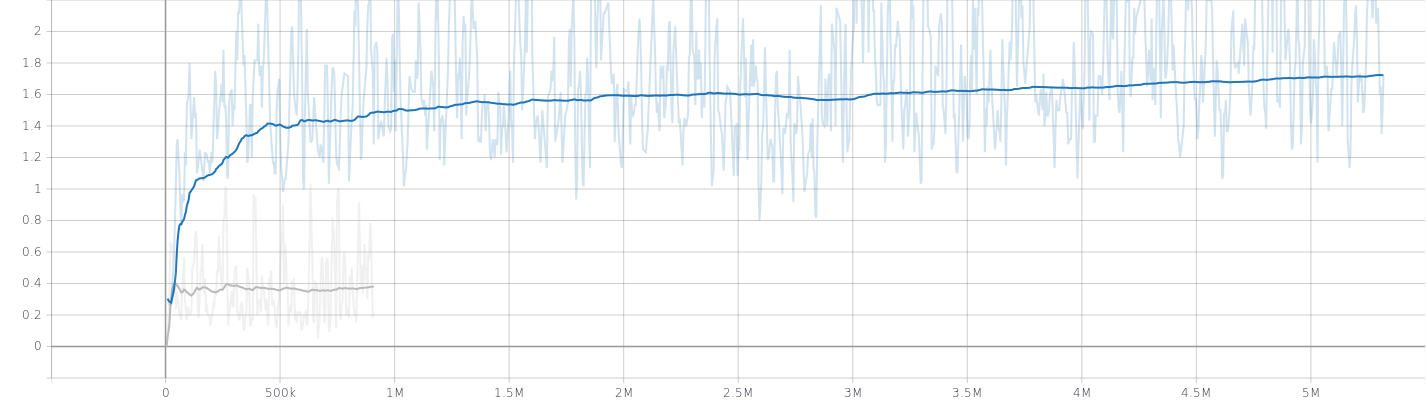
\includegraphics{./img/114084663-b8619100-98b0-11eb-8002-249f71b21557.png}
\caption{Reward 1, renewing mushroom. Combined-observation agent long
run (blue) vs.~random agent run (grey), showing mean reward score.
Smoothed graph.}
\end{figure}

\begin{figure}
\centering
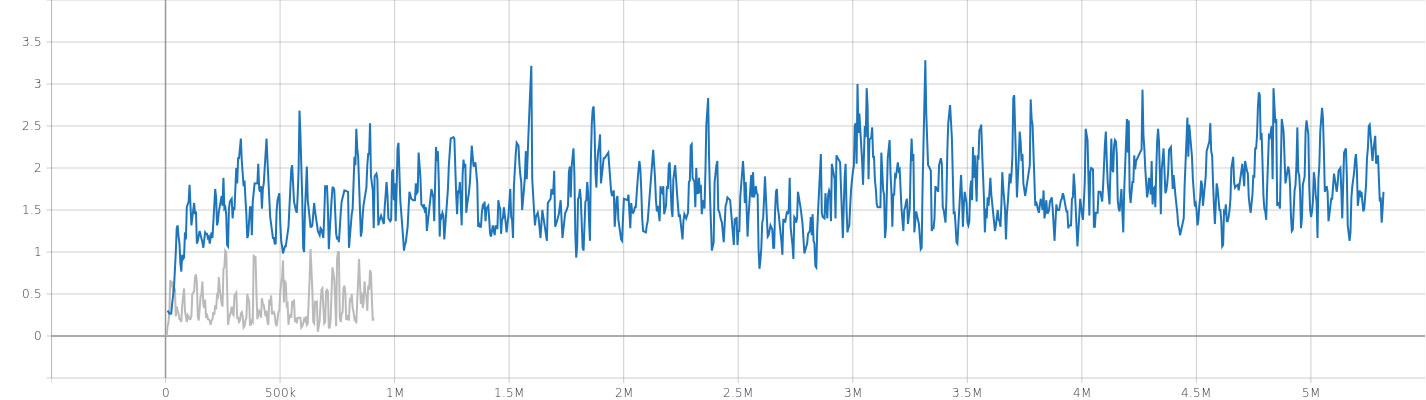
\includegraphics{./img/114084688-c31c2600-98b0-11eb-8a95-6bfd7e690953.png}
\caption{Reward 1, renewing mushroom. Combined-observation agent long
run (blue) vs.~random agent run (grey), showing mean reward score. Not
smoothed graph.}
\end{figure}

\begin{figure}
\centering
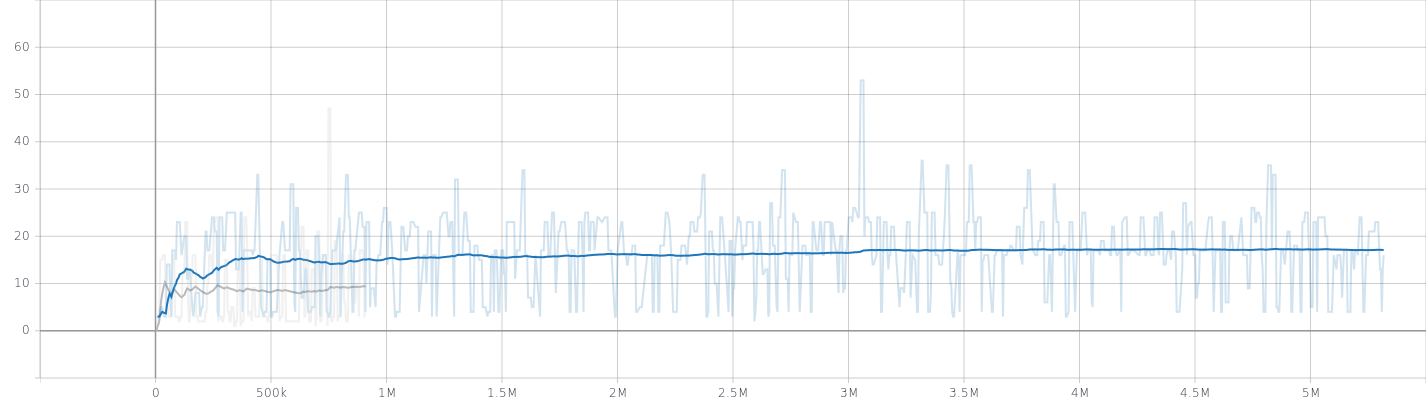
\includegraphics{./img/114084904-f9f23c00-98b0-11eb-9dc2-b08e4751a74f.png}
\caption{Reward 1, renewing mushroom. Combined-observation agent long
run (blue) vs.~random agent run (grey), showing max reward score.
Smoothed graph.}
\end{figure}

\begin{figure}
\centering
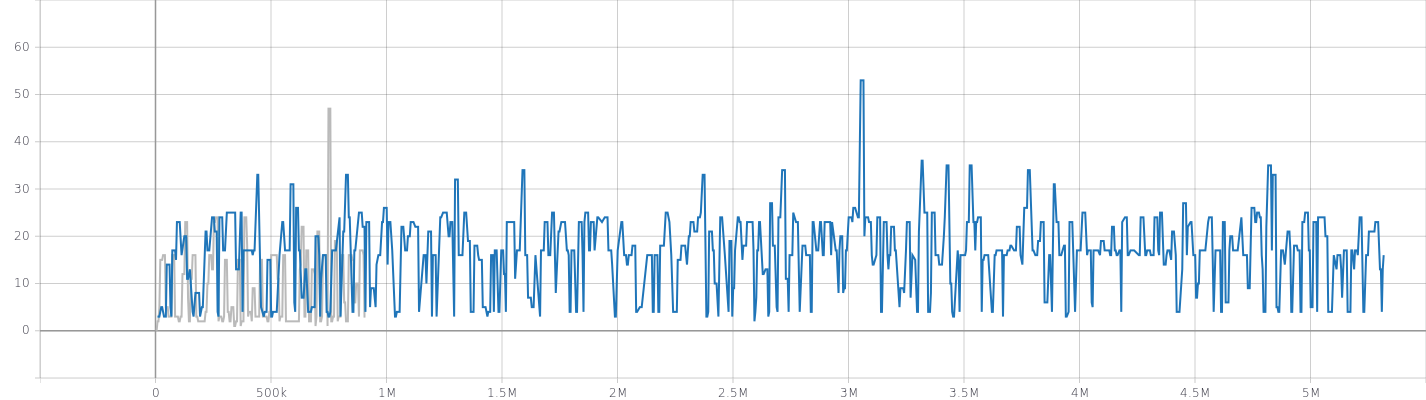
\includegraphics{./img/114084936-02e30d80-98b1-11eb-82b6-87b116a9bbd9.png}
\caption{Reward 1, renewing mushroom. Combined-observation agent long
run (blue) vs.~random agent run (grey), showing max reward score. Not
smoothed graph.}
\end{figure}

\begin{figure}
\centering
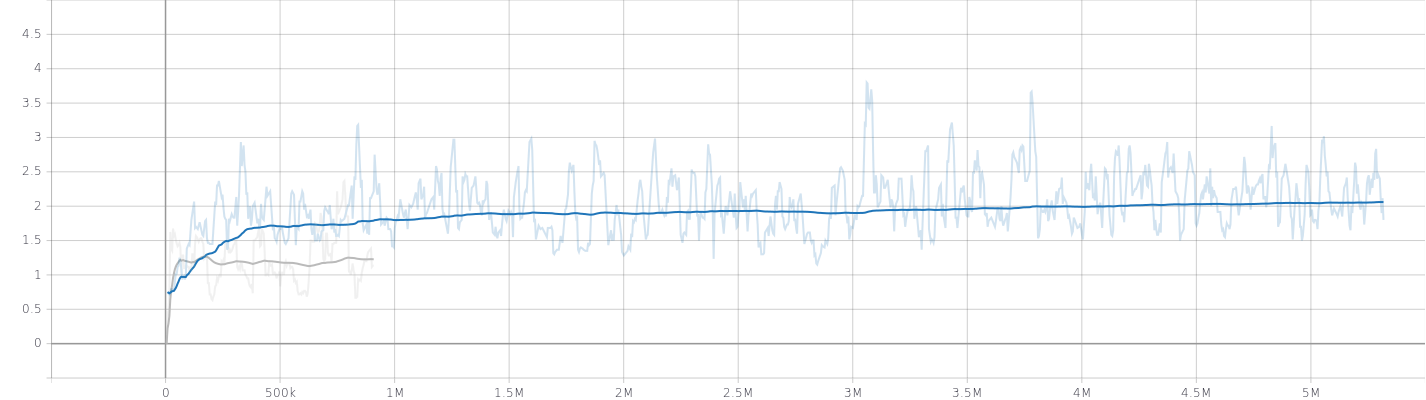
\includegraphics{./img/114084741-d0391500-98b0-11eb-9f85-bd11e5a799ae.png}
\caption{Reward 1, renewing mushroom. Combined-observation agent long
run (blue) vs.~random agent run (grey), showing mean escalated episodes
reward. Smoothed graph.}
\end{figure}

\begin{figure}
\centering
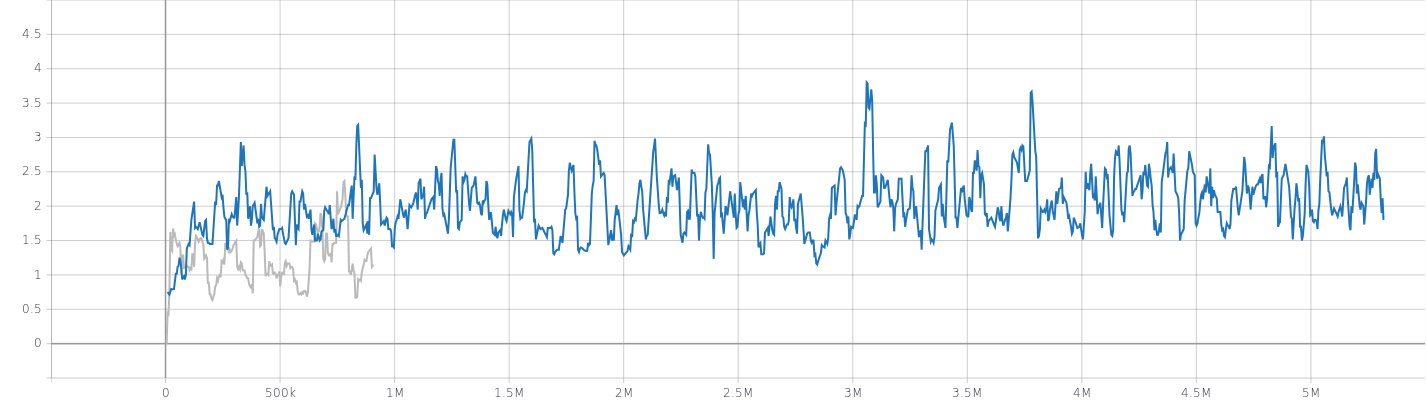
\includegraphics{./img/114084805-df1fc780-98b0-11eb-802c-6eb2f5d671f0.png}
\caption{Reward 1, renewing mushroom. Combined-observation agent long
run (blue) vs.~random agent run (grey), showing mean escalated episodes
reward. Not smoothed graph.}
\end{figure}

\begin{figure}
\centering
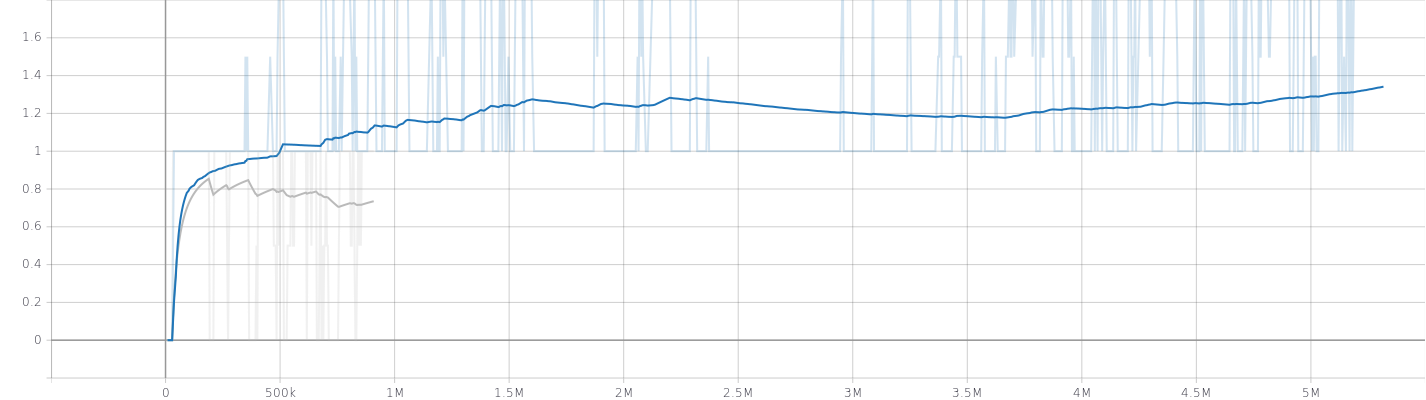
\includegraphics{./img/114091992-adf7c500-98b9-11eb-9bd1-6572f706ce9e.png}
\caption{Reward 1, renewing mushroom. Combined-observation agent long
run (blue) vs.~random agent run (grey), showing median escalated
episodes reward. Smoothed graph.}
\end{figure}

\begin{figure}
\centering
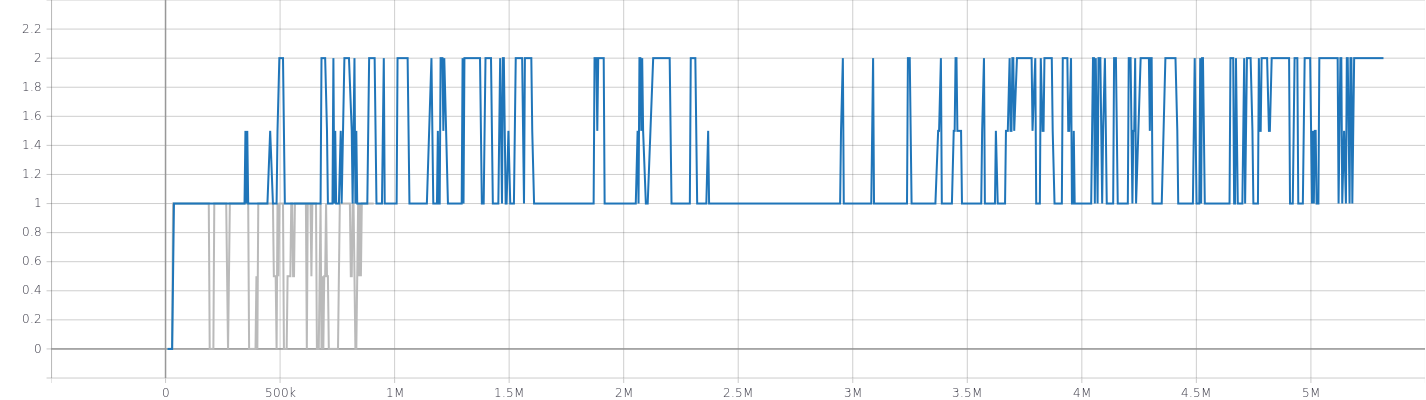
\includegraphics{./img/114092068-c071fe80-98b9-11eb-8806-7ce21effd1da.png}
\caption{Reward 1, renewing mushroom. Combined-observation agent long
run (blue) vs.~random agent run (grey), showing median escalated
episodes reward. Not smoothed graph.}
\end{figure}

\begin{figure}
\centering
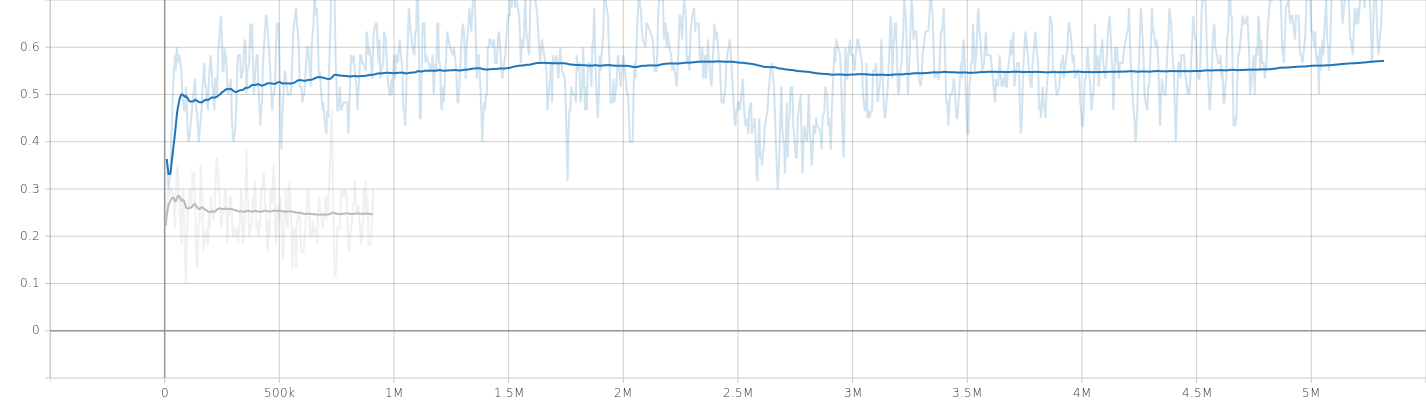
\includegraphics{./img/114084845-e941c600-98b0-11eb-92ac-cf469b25d135.png}
\caption{Reward 1, renewing mushroom. Combined-observation agent long
run (blue) vs.~random agent run (grey), showing escalated episodes
frequency. Smoothed graph.}
\end{figure}

\begin{figure}
\centering
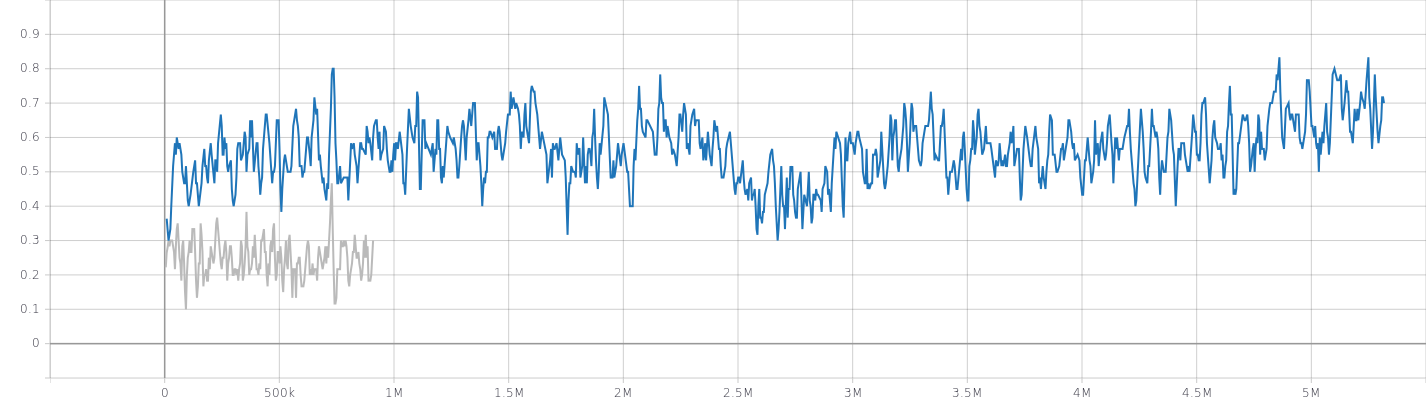
\includegraphics{./img/114084866-ef37a700-98b0-11eb-88e4-a81ebb4dae53.png}
\caption{Reward 1, renewing mushroom. Combined-observation agent long
run (blue) vs.~random agent run (grey), showing escalated episodes
frequency. Not smoothed graph.}
\end{figure}

\begin{figure}
\centering
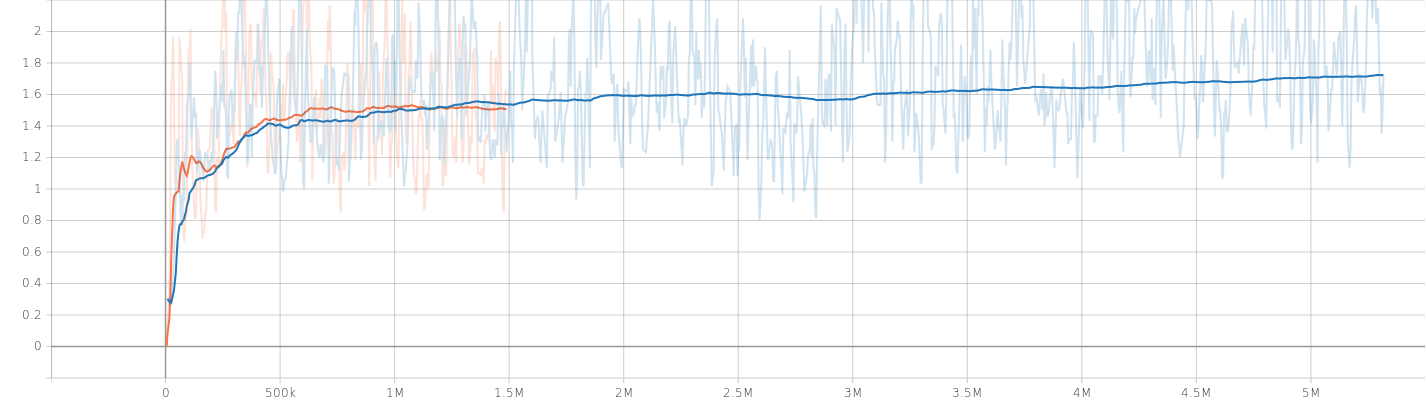
\includegraphics{./img/114085622-e4314680-98b1-11eb-9c94-fee1d1136a3b.png}
\caption{Reward 1, renewing mushroom. Combined-observation agent long
run (blue) vs.~pixel observation agent run (irange), showing mean reward
score. Smoothed graph.}
\end{figure}

\begin{figure}
\centering
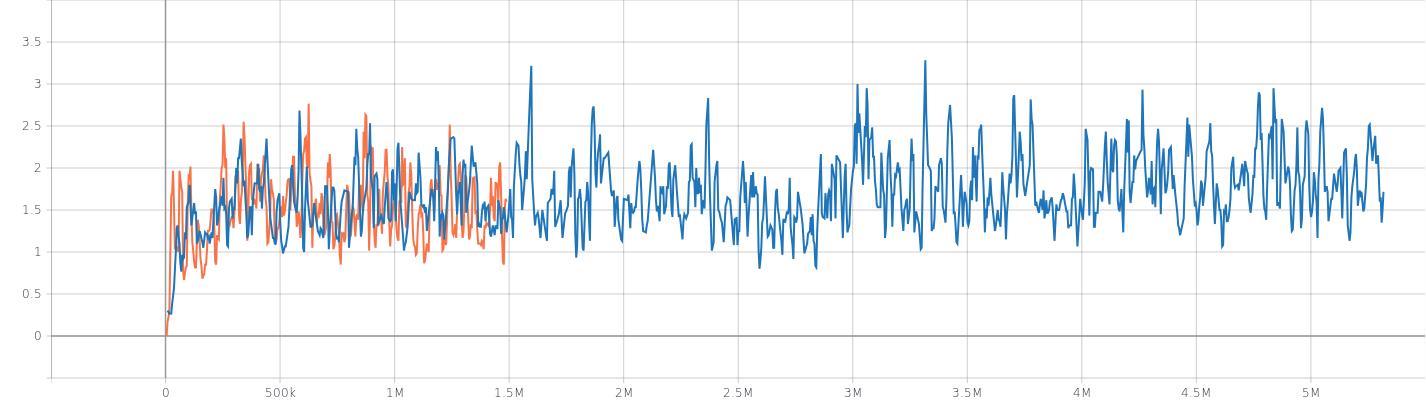
\includegraphics{./img/114085753-104cc780-98b2-11eb-837d-6426436cc838.png}
\caption{Reward 1, renewing mushroom. Combined-observation agent long
run (blue) vs.~pixel observation agent run (irange), showing mean reward
score. Not smoothed graph.}
\end{figure}

\begin{figure}
\centering
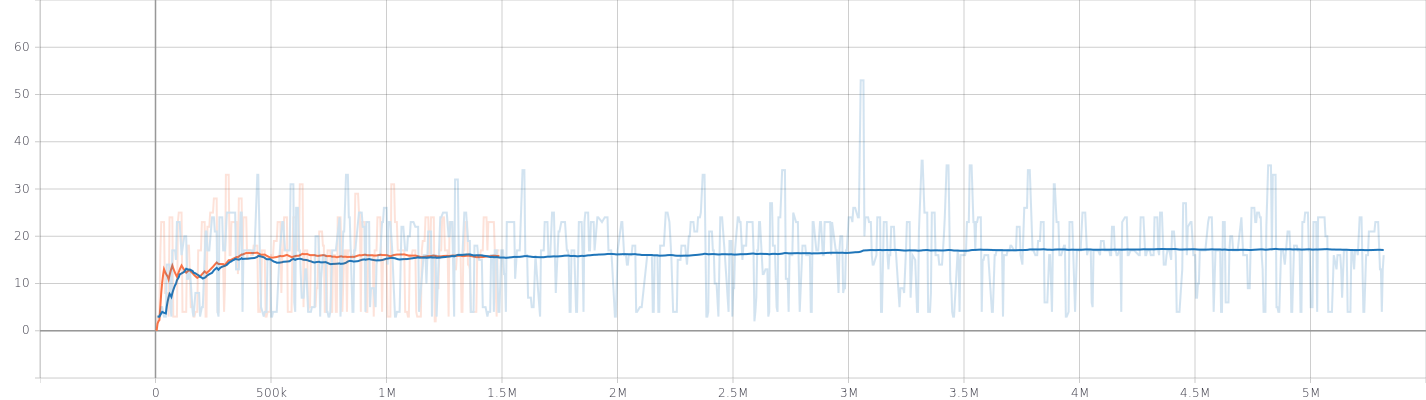
\includegraphics{./img/114086014-67529c80-98b2-11eb-82e1-34d404e5a999.png}
\caption{Reward 1, renewing mushroom. Combined-observation agent long
run (blue) vs.~pixel observation agent run (irange), showing max reward
score. Smoothed graph.}
\end{figure}

\begin{figure}
\centering
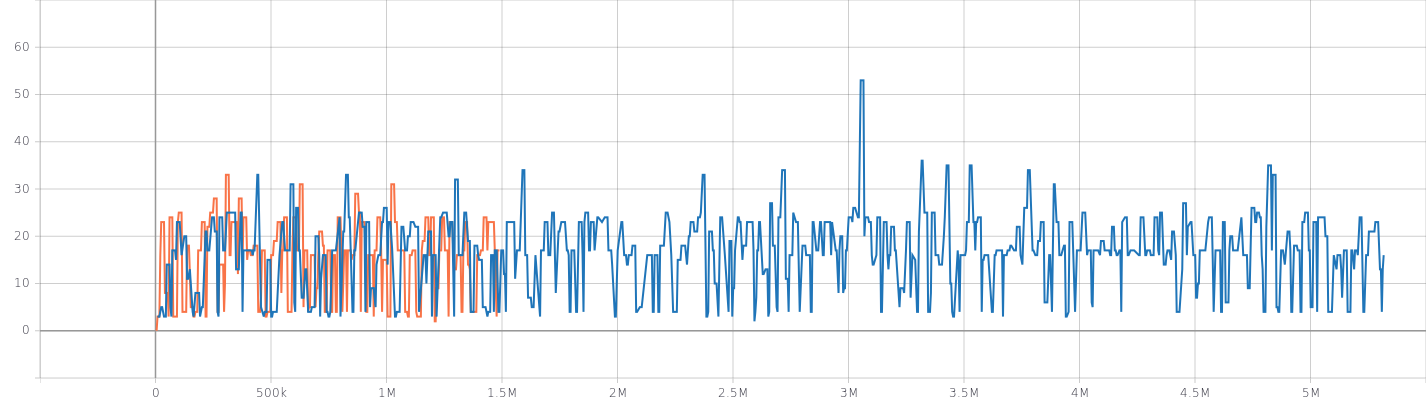
\includegraphics{./img/114086048-6faad780-98b2-11eb-8c0e-764396b1fc3b.png}
\caption{Reward 1, renewing mushroom. Combined-observation agent long
run (blue) vs.~pixel observation agent run (irange), showing max reward
score. Not smoothed graph.}
\end{figure}

\begin{figure}
\centering
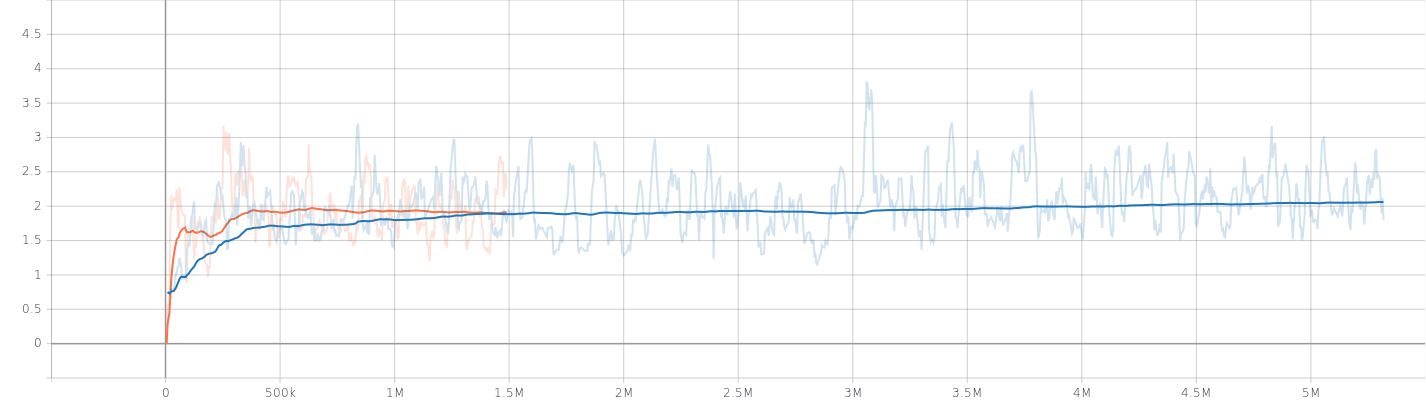
\includegraphics{./img/114085778-18a50280-98b2-11eb-804c-ea5656675625.png}
\caption{Reward 1, renewing mushroom. Combined-observation agent long
run (blue) vs.~pixel observation agent run (irange), showing mean
escalated episodes reward. Smoothed graph.}
\end{figure}

\begin{figure}
\centering
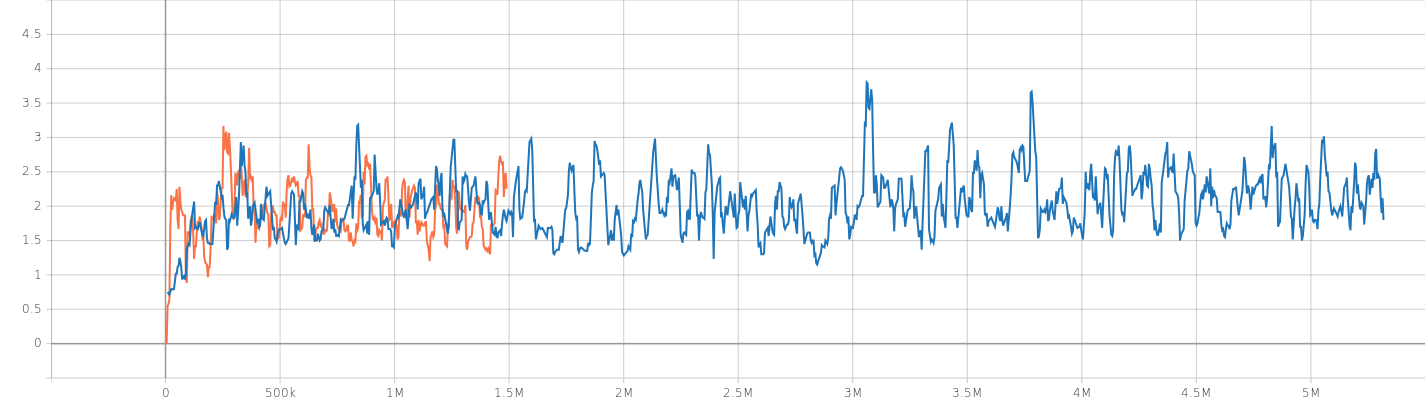
\includegraphics{./img/114085813-2490c480-98b2-11eb-8abb-0a5477ab4140.png}
\caption{Reward 1, renewing mushroom. Combined-observation agent long
run (blue) vs.~pixel observation agent run (irange), showing mean
escalated episodes reward. Not smoothed graph.}
\end{figure}

\begin{figure}
\centering
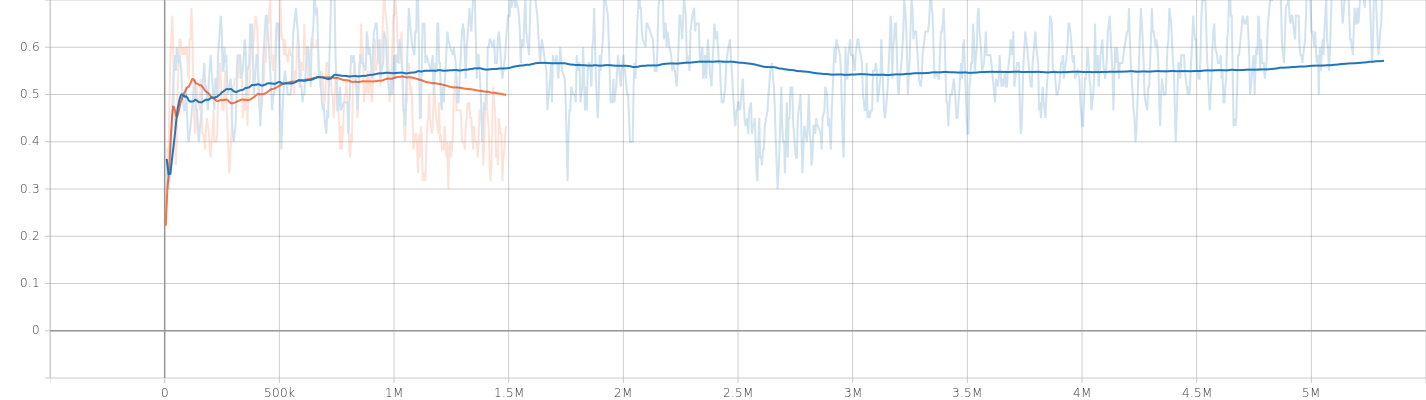
\includegraphics{./img/114085848-31adb380-98b2-11eb-8d23-7ab1e36eae2a.png}
\caption{Reward 1, renewing mushroom. Combined-observation agent long
run (blue) vs.~pixel observation agent run (irange), showing escalated
episodes frequency. Smoothed graph.}
\end{figure}

\begin{figure}
\centering
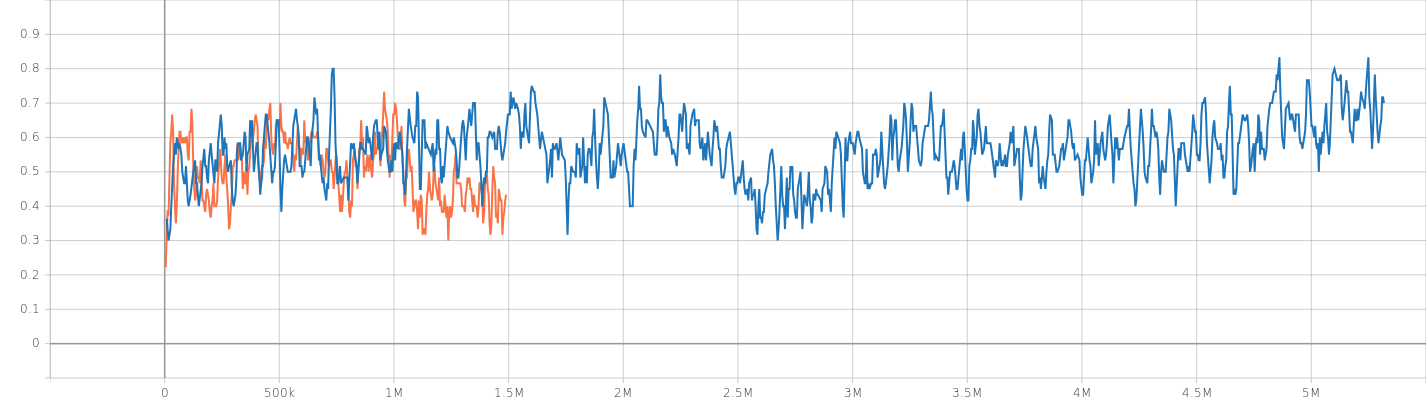
\includegraphics{./img/114085952-543fcc80-98b2-11eb-924b-a9e7ebf03cac.png}
\caption{Reward 1, renewing mushroom. Combined-observation agent long
run (blue) vs.~pixel observation agent run (irange), showing escalated
episodes frequency. Not smoothed graph.}
\end{figure}

\begin{figure}
\centering
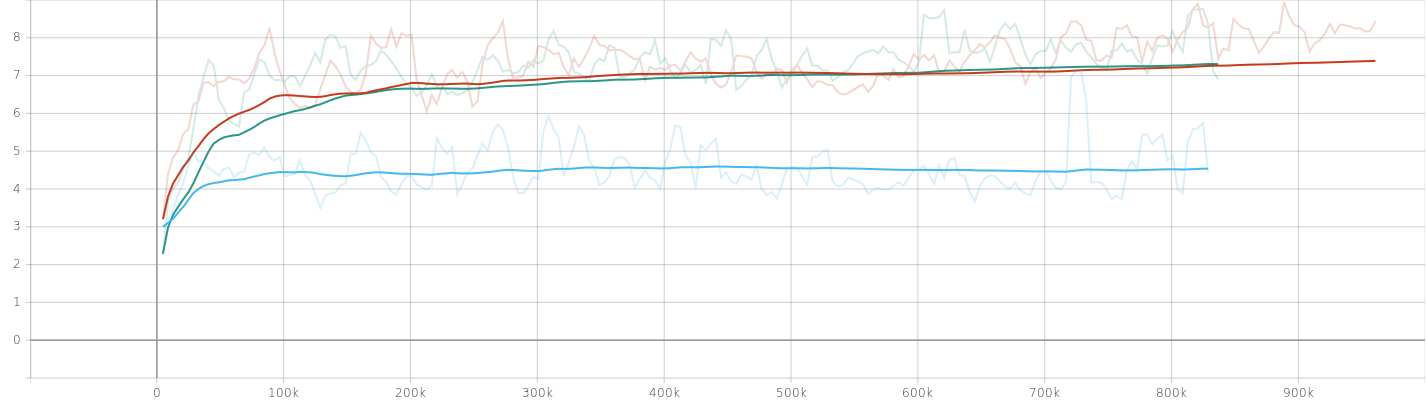
\includegraphics{./img/114086669-2f982480-98b3-11eb-91db-ff7f9dbdc092.png}
\caption{Reward 3, renewing mushroom. Combined-observation agent runs
(red, green) vs.~random agent run (light blue), showing mean reward
score. Smoothed graph.}
\end{figure}

\begin{figure}
\centering
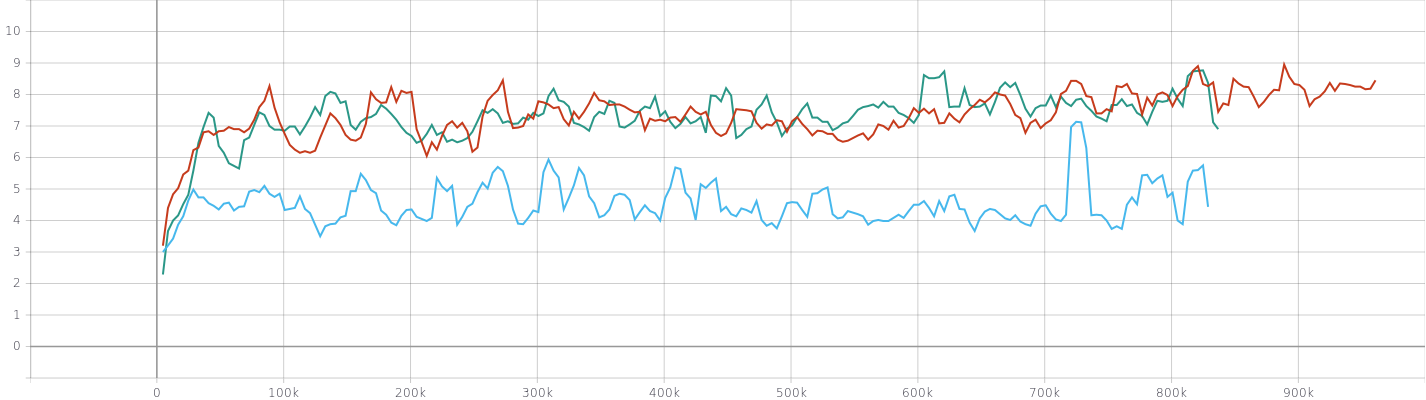
\includegraphics{./img/114086692-3757c900-98b3-11eb-9956-8999f0431ddf.png}
\caption{Reward 3, renewing mushroom. Combined-observation agent runs
(red, green) vs.~random agent run (light blue), showing mean reward
score. Not smoothed graph.}
\end{figure}

\begin{figure}
\centering
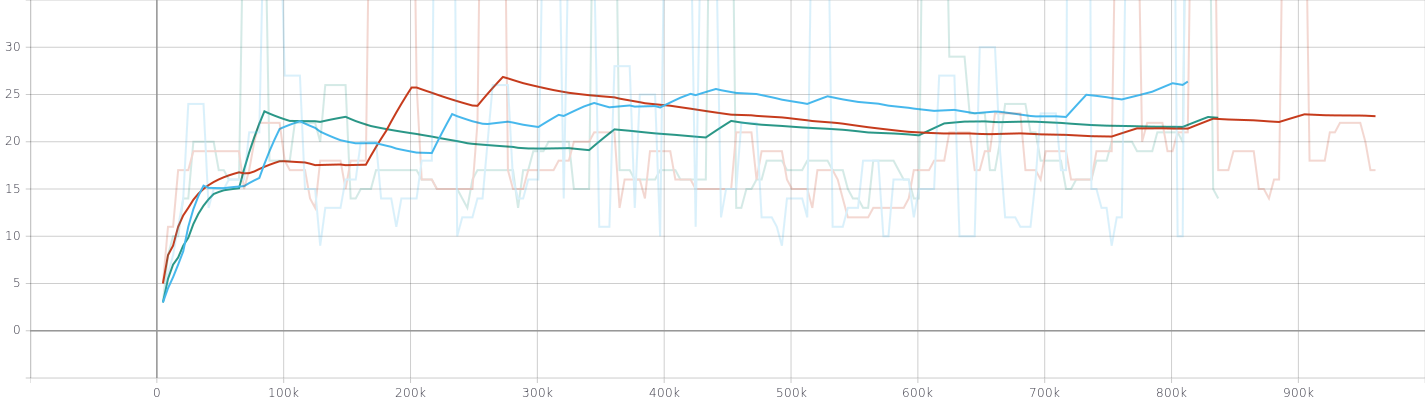
\includegraphics{./img/114086784-57878800-98b3-11eb-97db-628db56a8d7d.png}
\caption{Reward 3, renewing mushroom. Combined-observation agent runs
(red, green) vs.~random agent run (light blue), showing max reward
score. Smoothed graph.}
\end{figure}

\begin{figure}
\centering
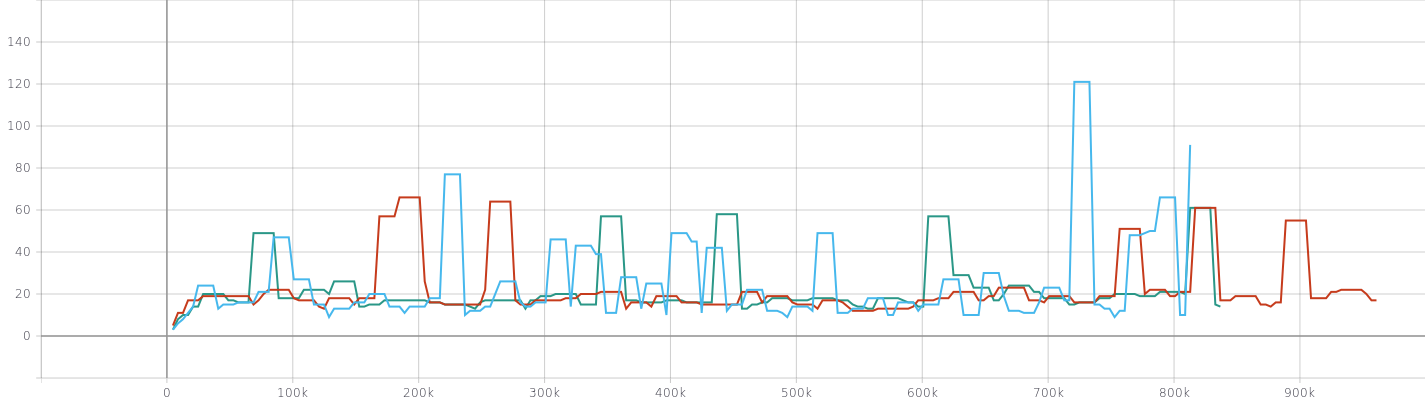
\includegraphics{./img/114086807-63734a00-98b3-11eb-9dfb-ed7871c8f18a.png}
\caption{Reward 3, renewing mushroom. Combined-observation agent runs
(red, green) vs.~random agent run (light blue), showing max reward
score. Not smoothed graph.}
\end{figure}

\begin{figure}
\centering
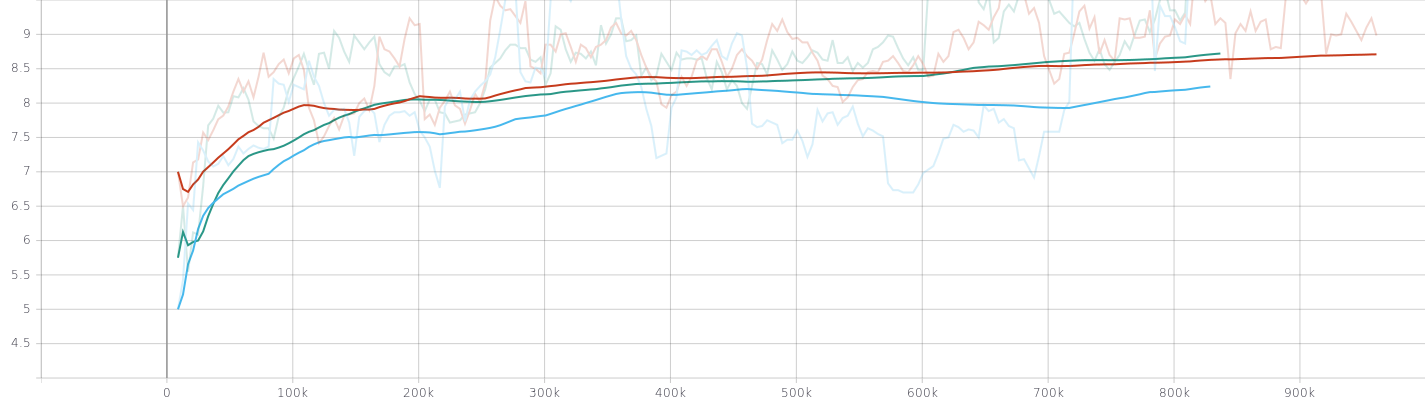
\includegraphics{./img/114086864-784fdd80-98b3-11eb-9080-b71419e86321.png}
\caption{Reward 3, renewing mushroom. Combined-observation agent runs
(red, green) vs.~random agent run (light blue), showing mean escalated
episodes reward. Smoothed graph.}
\end{figure}

\begin{figure}
\centering
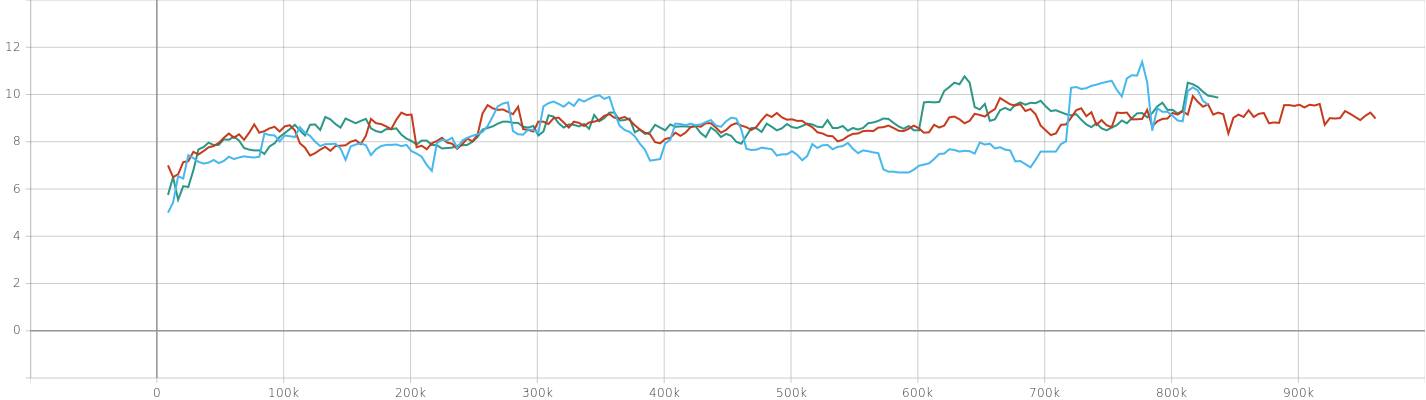
\includegraphics{./img/114087064-b220e400-98b3-11eb-8ef1-881c796127f4.png}
\caption{Reward 3, renewing mushroom. Combined-observation agent runs
(red, green) vs.~random agent run (light blue), showing mean escalated
episodes reward. Not smoothed graph.}
\end{figure}

\begin{figure}
\centering
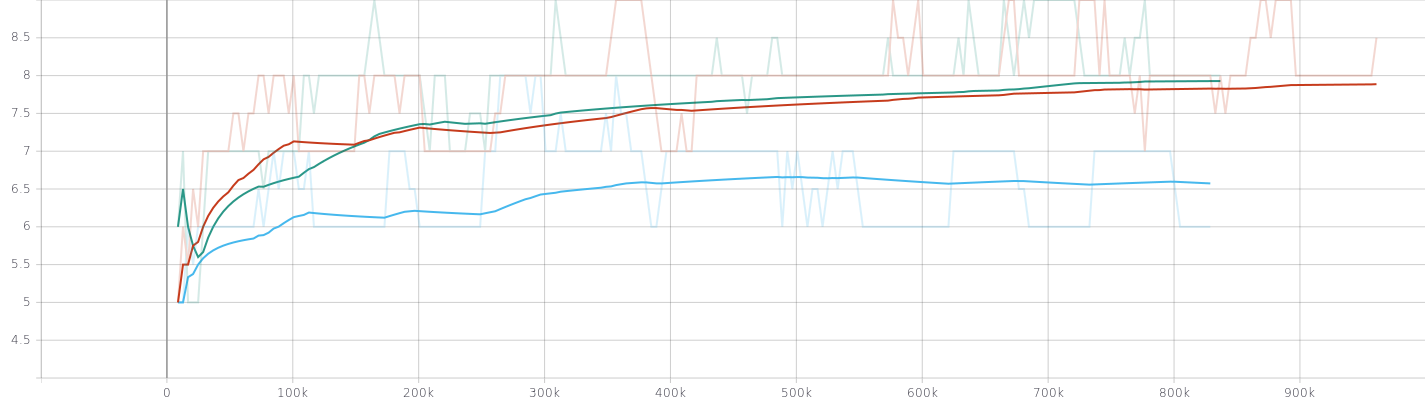
\includegraphics{./img/114091488-0da1a080-98b9-11eb-9123-f7a314085a8b.png}
\caption{Reward 3, renewing mushroom. Combined-observation agent runs
(red, green) vs.~random agent run (light blue), showing median escalated
episodes reward. Smoothed graph.}
\end{figure}

\begin{figure}
\centering
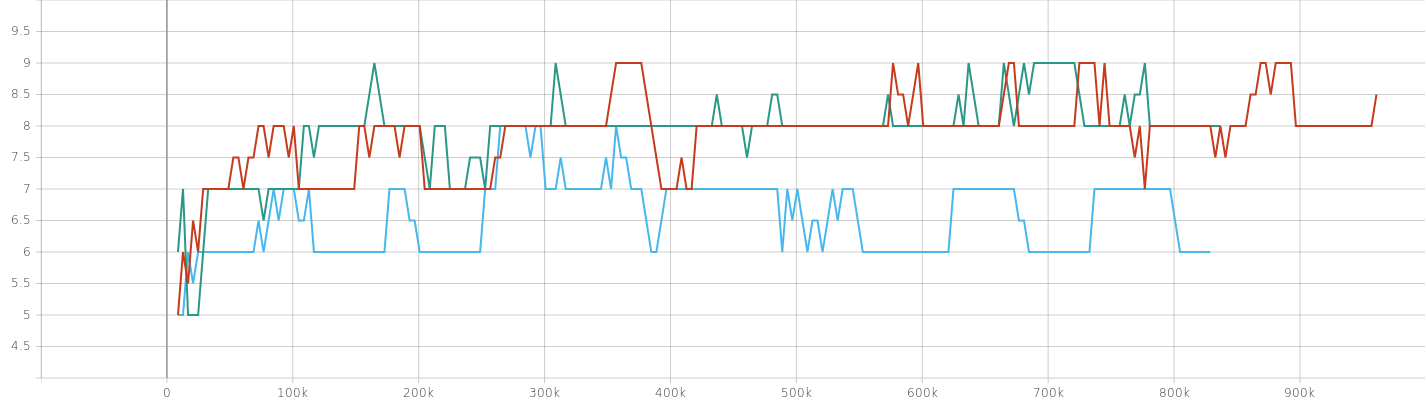
\includegraphics{./img/114091547-1eeaad00-98b9-11eb-94cf-fcbcccb5a9df.png}
\caption{Reward 3, renewing mushroom. Combined-observation agent runs
(red, green) vs.~random agent run (light blue), showing median escalated
episodes reward. Not smoothed graph.}
\end{figure}

\begin{figure}
\centering
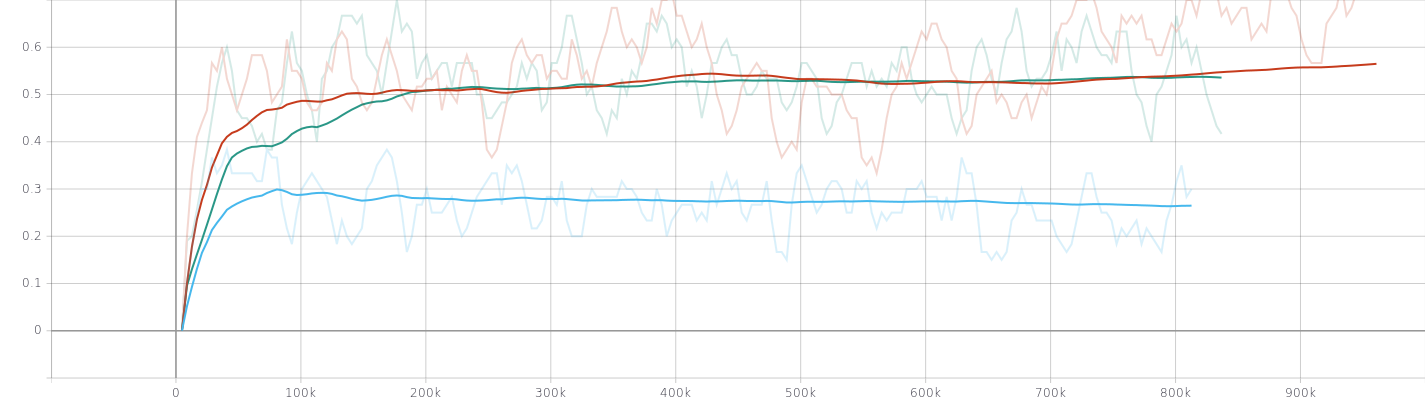
\includegraphics{./img/114087180-d67cc080-98b3-11eb-84e5-29246fdaff00.png}
\caption{Reward 3, renewing mushroom. Combined-observation agent runs
(red, green) vs.~random agent run (light blue), showing escalated
episodes frequency. Smoothed graph.}
\end{figure}

\begin{figure}
\centering
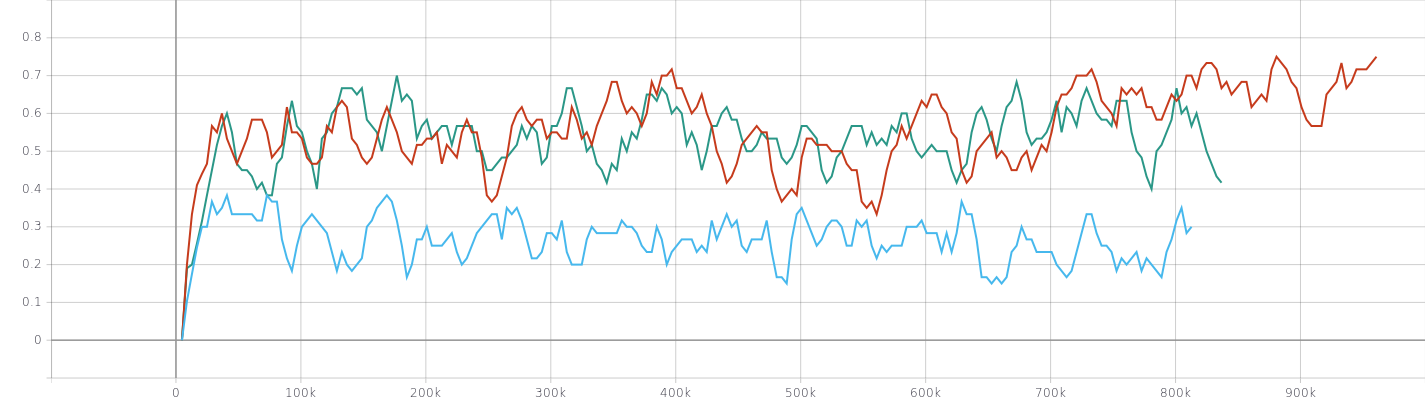
\includegraphics{./img/114087274-f8764300-98b3-11eb-8c0a-6a45d264176d.png}
\caption{Reward 3, renewing mushroom. Combined-observation agent runs
(red, green) vs.~random agent run (light blue), showing escalated
episodes frequency. Not smoothed graph.}
\end{figure}

\begin{figure}
\centering
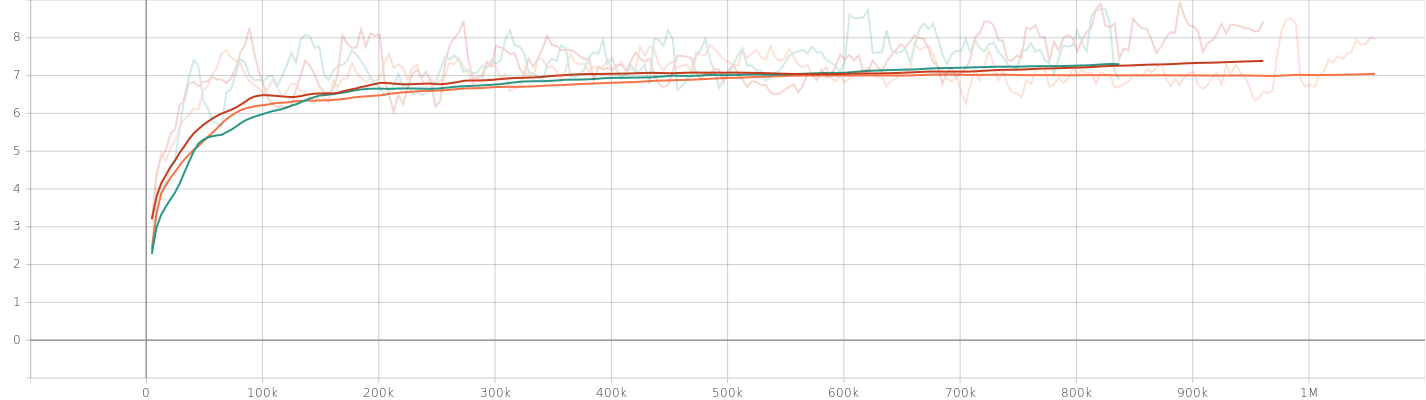
\includegraphics{./img/114088707-94ed1500-98b5-11eb-828d-5b2b6e865df1.png}
\caption{Reward 3, renewing mushroom. Combined-observation agent runs
(greed, red) vs.~pixel observation agent run (orange), showing mean
reward score. Smoothed graph.}
\end{figure}

\begin{figure}
\centering
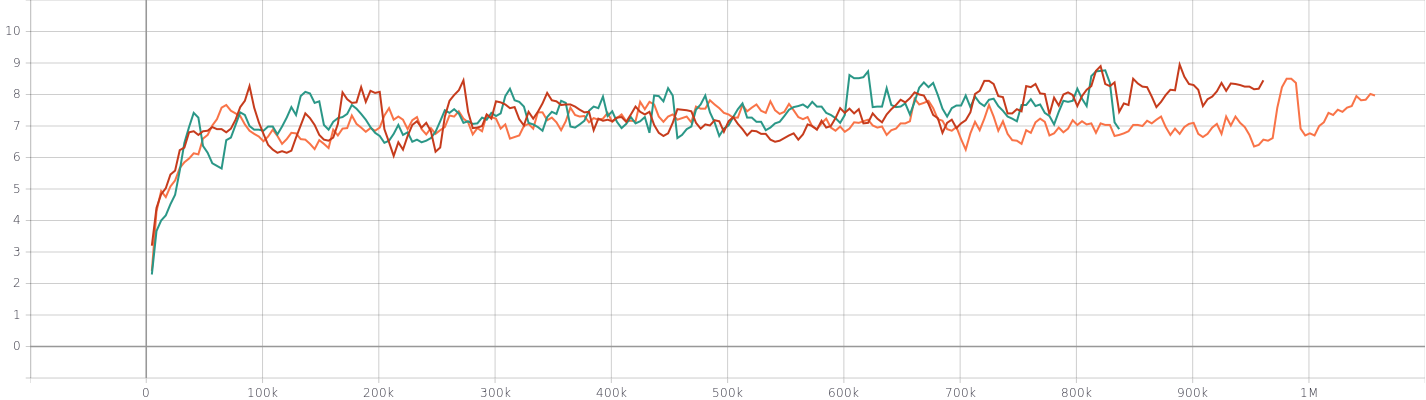
\includegraphics{./img/114088887-ce258500-98b5-11eb-9f24-b3dba2022036.png}
\caption{Reward 3, renewing mushroom. Combined-observation agent runs
(greed, red) vs.~pixel observation agent run (orange), showing mean
reward score. Not smoothed graph.}
\end{figure}

\begin{figure}
\centering
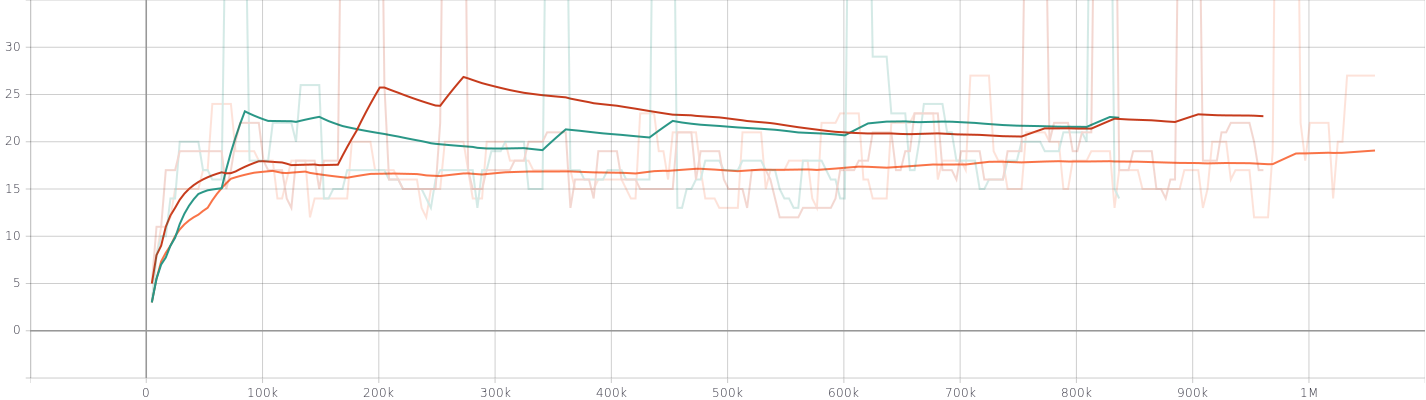
\includegraphics{./img/114088967-e4334580-98b5-11eb-9ba0-958450ed4f54.png}
\caption{Reward 3, renewing mushroom. Combined-observation agent runs
(greed, red) vs.~pixel observation agent run (orange), showing max
reward score. Smoothed graph.}
\end{figure}

\begin{figure}
\centering
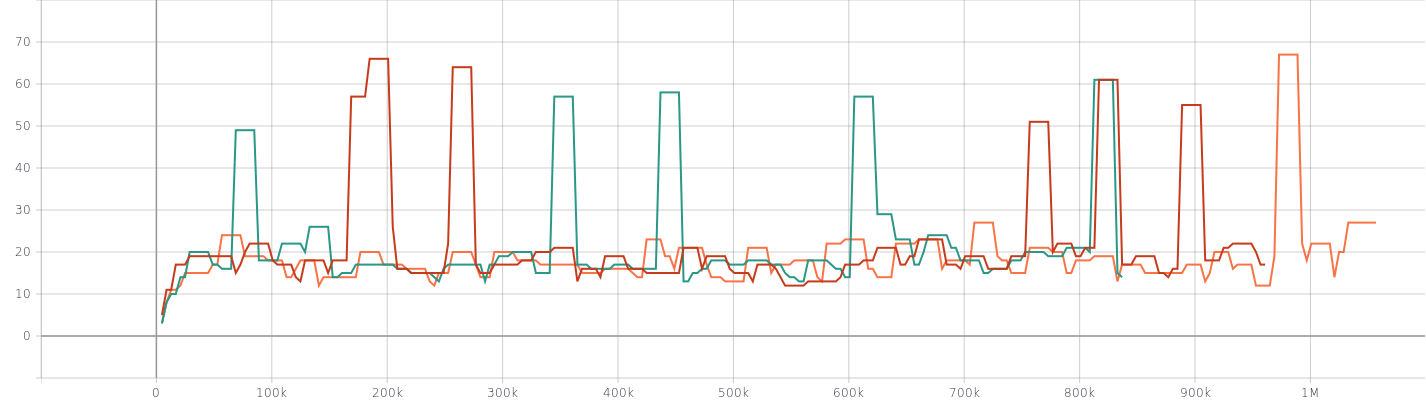
\includegraphics{./img/114088996-edbcad80-98b5-11eb-8ac5-273586752b65.png}
\caption{Reward 3, renewing mushroom. Combined-observation agent runs
(greed, red) vs.~pixel observation agent run (orange), showing max
reward score. Not smoothed graph.}
\end{figure}

\begin{figure}
\centering
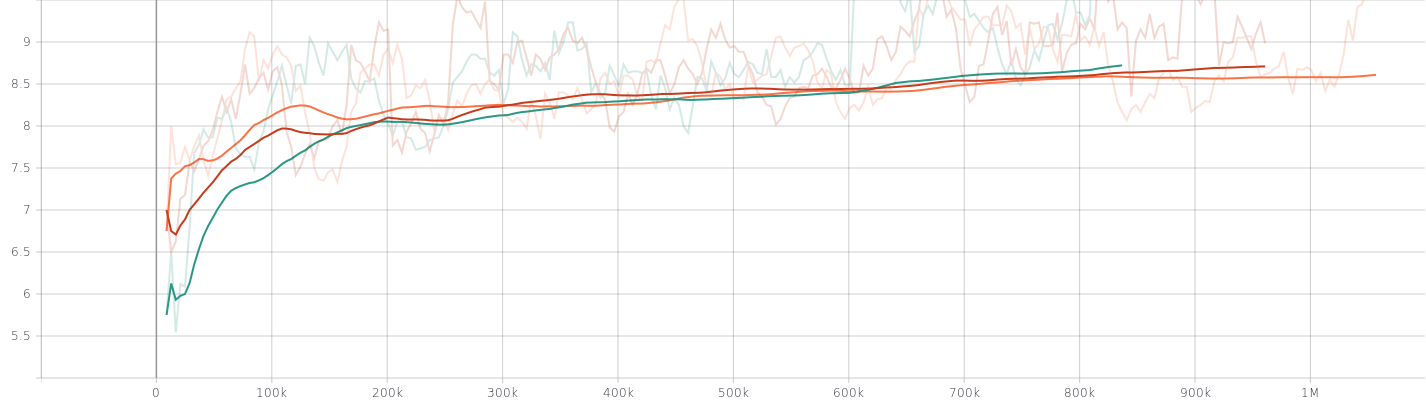
\includegraphics{./img/114089048-fd3bf680-98b5-11eb-868b-8b4eb53b3287.png}
\caption{Reward 3, renewing mushroom. Combined-observation agent runs
(greed, red) vs.~pixel observation agent run (orange), showing mean
escalated episodes reward. Smoothed graph.}
\end{figure}

\begin{figure}
\centering
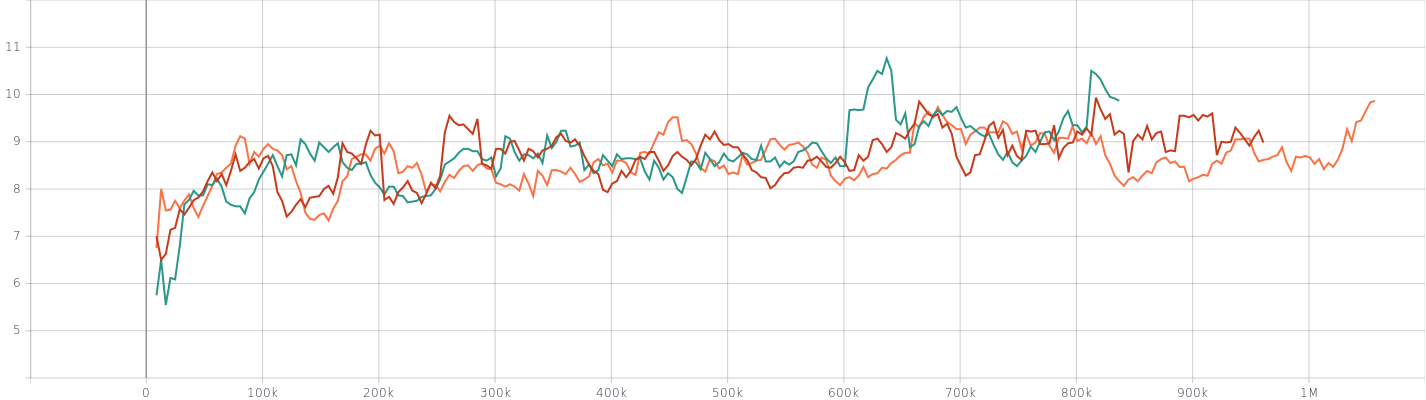
\includegraphics{./img/114089086-06c55e80-98b6-11eb-8bcd-c67011250e6e.png}
\caption{Reward 3, renewing mushroom. Combined-observation agent runs
(greed, red) vs.~pixel observation agent run (orange), showing mean
escalated episodes reward. Not smoothed graph.}
\end{figure}

\begin{figure}
\centering
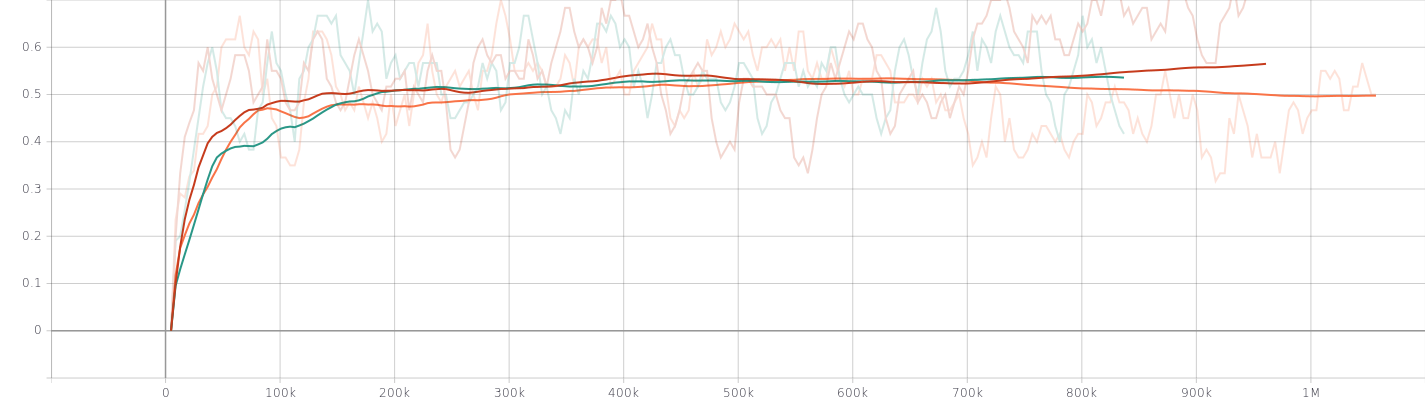
\includegraphics{./img/114089128-12188a00-98b6-11eb-9f61-a544f493a2f0.png}
\caption{Reward 3, renewing mushroom. Combined-observation agent runs
(greed, red) vs.~pixel observation agent run (orange), showing escalated
episodes frequency. Smoothed graph.}
\end{figure}

\begin{figure}
\centering
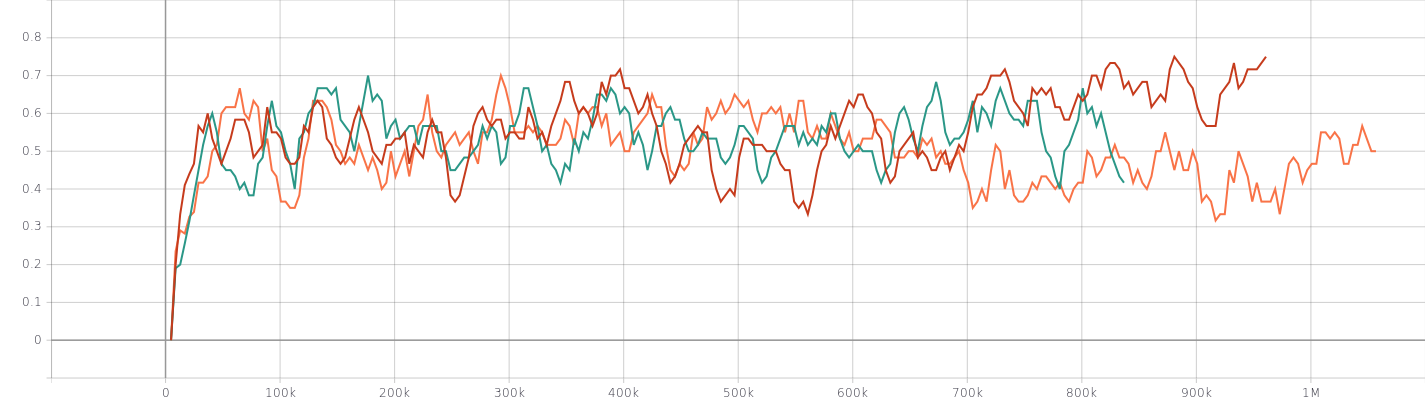
\includegraphics{./img/114089168-1c3a8880-98b6-11eb-9420-669eec175369.png}
\caption{Reward 3, renewing mushroom. Combined-observation agent runs
(greed, red) vs.~pixel observation agent run (orange), showing escalated
episodes frequency. Not smoothed graph.}
\end{figure}

\begin{figure}
\centering
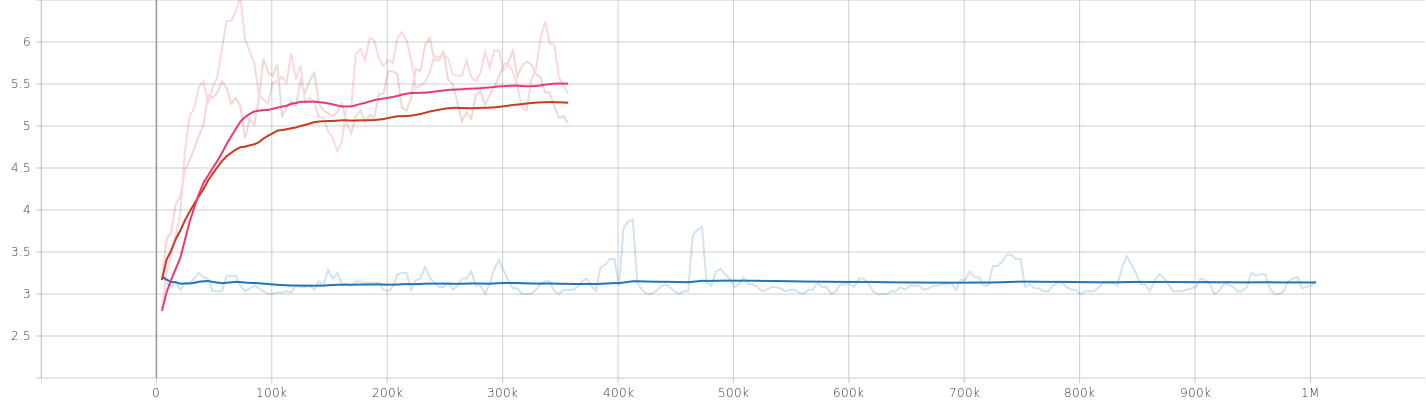
\includegraphics{./img/114090885-49883600-98b8-11eb-90cf-b0244b0fbc63.png}
\caption{Reward 3, single mushroom. Combined-observation agent runs
(magenta, red) vs.~large random agent run (blue), showing mean reward
score. Smoothed graph.}
\end{figure}

\begin{figure}
\centering
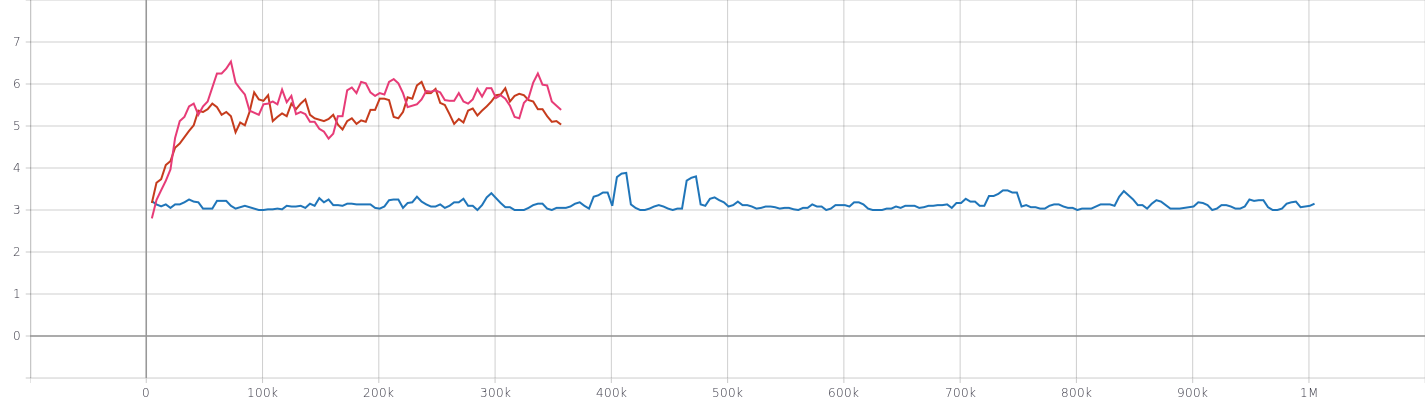
\includegraphics{./img/114090937-57d65200-98b8-11eb-8449-ed66b1f58fc3.png}
\caption{Reward 3, single mushroom. Combined-observation agent runs
(magenta, red) vs.~large random agent run (blue), showing mean reward
score. Not smoothed graph.}
\end{figure}

\begin{figure}
\centering
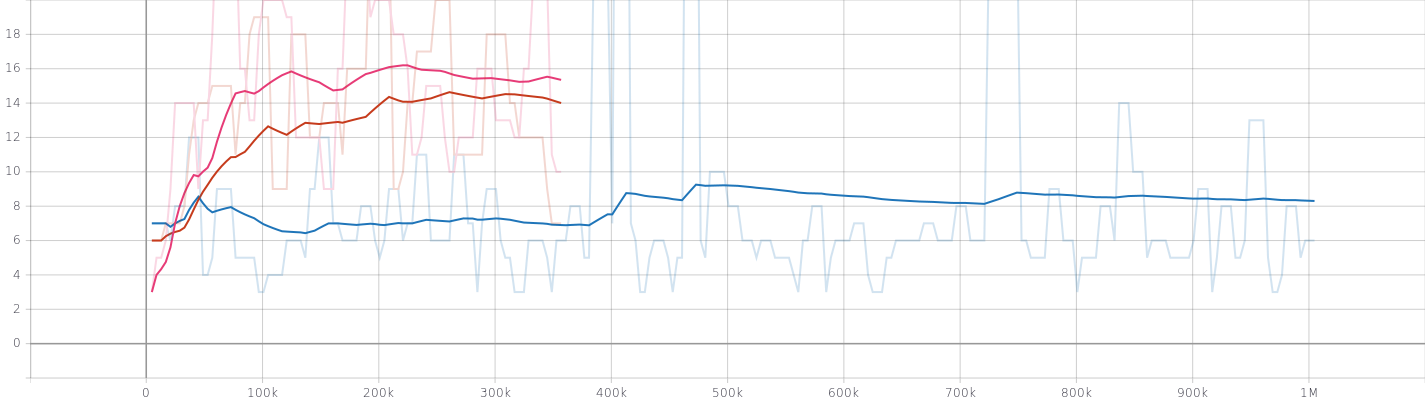
\includegraphics{./img/114090517-d4b4fc00-98b7-11eb-969b-e0598c294397.png}
\caption{Reward 3, single mushroom. Combined-observation agent runs
(magenta, red) vs.~large random agent run (blue), showing max reward
score. Smoothed graph.}
\end{figure}

\begin{figure}
\centering
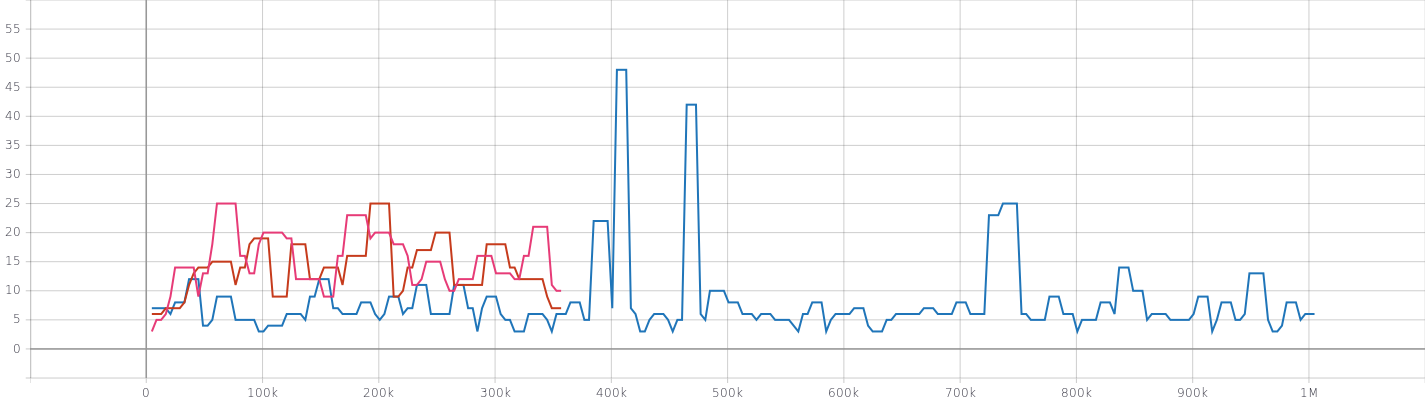
\includegraphics{./img/114090547-dd0d3700-98b7-11eb-83b5-9127ac49814b.png}
\caption{Reward 3, single mushroom. Combined-observation agent runs
(magenta, red) vs.~large random agent run (blue), showing max reward
score. Not smoothed graph.}
\end{figure}

\begin{figure}
\centering
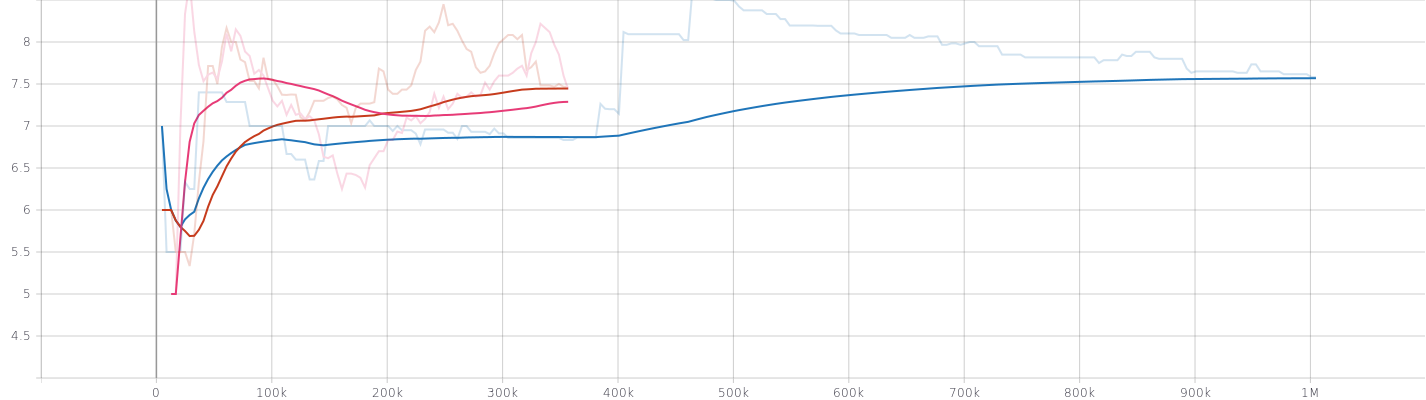
\includegraphics{./img/114090659-0201aa00-98b8-11eb-9b32-1d111a988ecb.png}
\caption{Reward 3, single mushroom. Combined-observation agent runs
(magenta, red) vs.~large random agent run (blue), showing mean escalated
episodes reward. Smoothed graph.}
\end{figure}

\begin{figure}
\centering
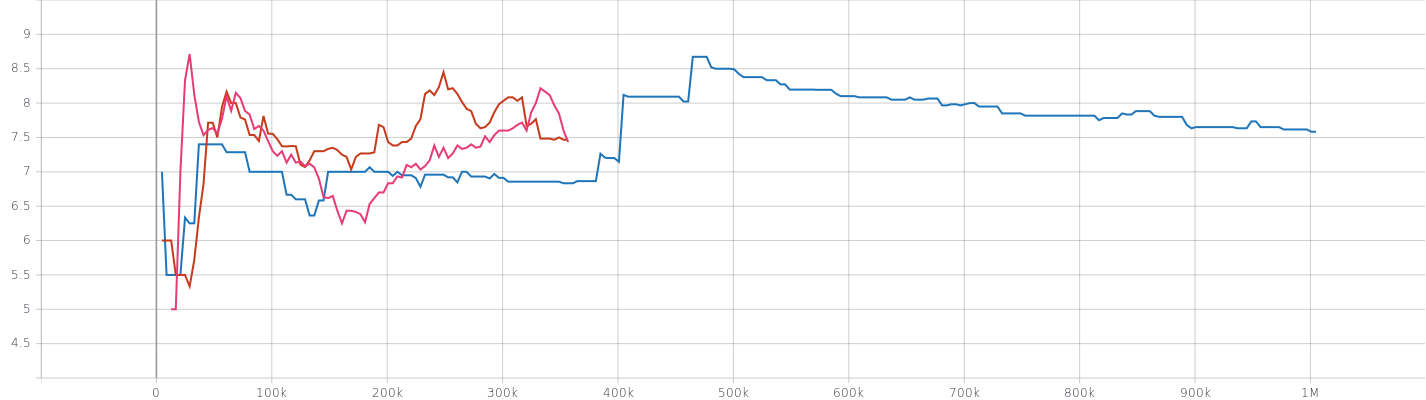
\includegraphics{./img/114090695-0c23a880-98b8-11eb-9e70-874fcbd055fb.png}
\caption{Reward 3, single mushroom. Combined-observation agent runs
(magenta, red) vs.~large random agent run (blue), showing mean escalated
episodes reward. Not smoothed graph.}
\end{figure}

\begin{figure}
\centering
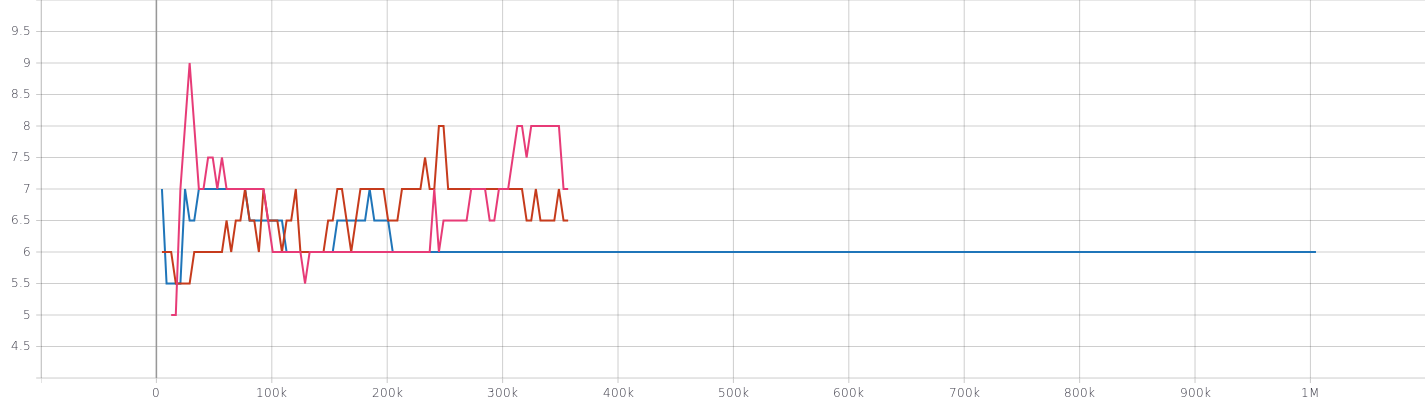
\includegraphics{./img/last-exper-median-crash-reward-rough.png}
\caption{Reward 3, single mushroom. Combined-observation agent runs
(magenta, red) vs.~large random agent run (blue), showing median
escalated episodes reward. Smoothed graph.}
\end{figure}

\begin{figure}
\centering
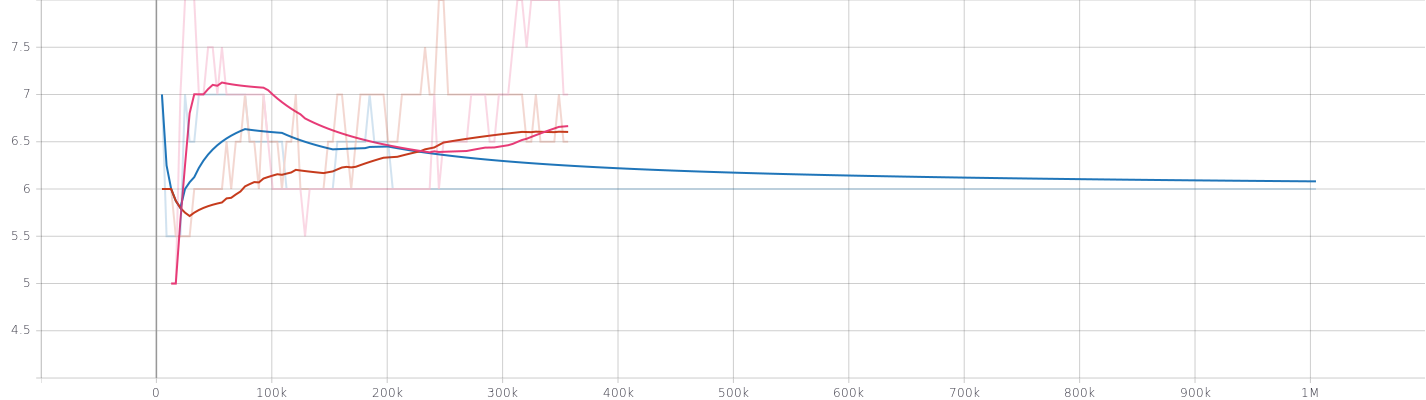
\includegraphics{./img/last-exper-median-crash-reward-smooth.png}
\caption{Reward 3, single mushroom. Combined-observation agent runs
(magenta, red) vs.~large random agent run (blue), showing median
escalated episodes reward. Not smoothed graph.}
\end{figure}

\begin{figure}
\centering
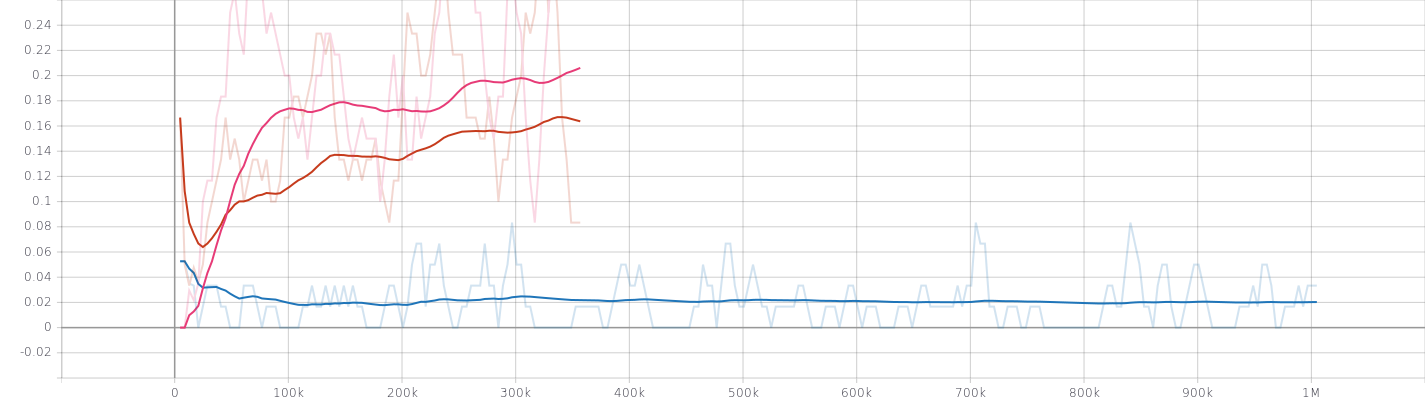
\includegraphics{./img/114090722-147be380-98b8-11eb-9a06-2831ef960127.png}
\caption{Reward 3, single mushroom. Combined-observation agent runs
(magenta, red) vs.~large random agent run (blue), showing escalated
episodes frequency. Smoothed graph.}
\end{figure}

\begin{figure}
\centering
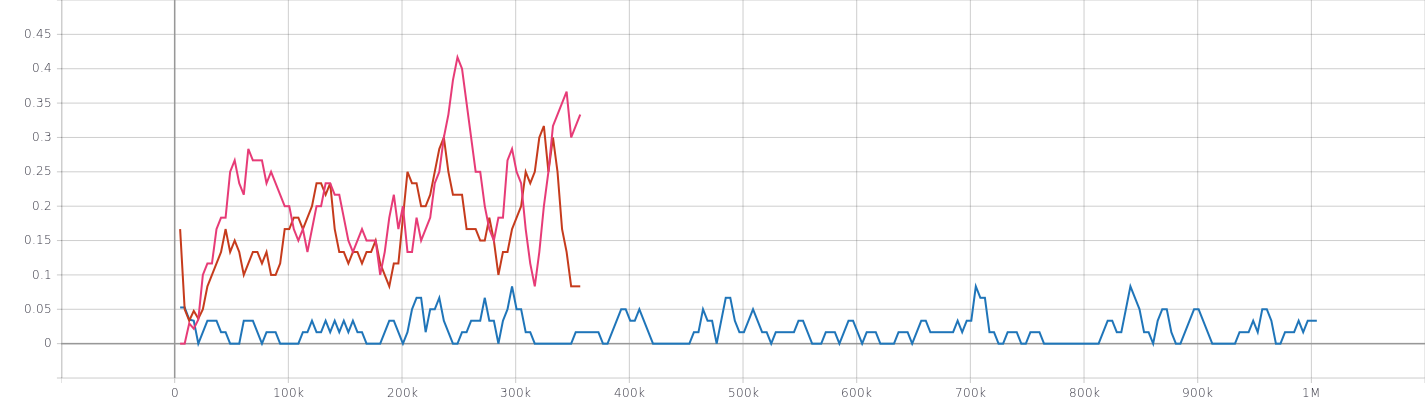
\includegraphics{./img/114090782-28bfe080-98b8-11eb-9912-6b584a28ca75.png}
\caption{Reward 3, single mushroom. Combined-observation agent runs
(magenta, red) vs.~large random agent run (blue), showing escalated
episodes frequency. Not smoothed graph.}
\end{figure}

\begin{figure}
\centering

\includegraphics{./img/Tuesday-13-22-36.jpg}
\caption{Glass window effect.}
\end{figure}

\begin{figure}
\centering

\includegraphics{./img/Tuesday-13-24-52.jpg}
\caption{Black blocks.}
\end{figure}

\begin{figure}
\centering

\includegraphics{./img/Tuesday-13-25-46.jpg}
\caption{Sky jumbled with artifacts.}
\end{figure}

\begin{figure}
\centering
\includegraphics{./img/Tuesday-13-26-58.jpg}
\caption{Sky became pink.}
\end{figure}

\begin{figure}
\centering
\includegraphics{./img/Tuesday-13-28-43.jpg}
\caption{Screen filled with brown lump pattern.}
\end{figure}

\begin{figure}
\centering
\includegraphics{./img/Tuesday-13-33-50.jpg}
\caption{Blocks replaced with silhouette.}
\end{figure}

\begin{figure}
\centering
\includegraphics{./img/Tuesday-13-33-58.jpg}
\caption{Screen filled with green patterns.}
\end{figure}

\begin{figure}
\centering
\includegraphics{./img/Tuesday-13-36-07.jpg}
\caption{Chaos cascade: scenery sprites replaced with artifacts.}
\end{figure}

\begin{figure}
\centering
\includegraphics{./img/Tuesday-13-40-25.jpg}
\caption{Raining pows: sky replaced by pattern.}
\end{figure}

\begin{figure}
\centering
\includegraphics{./img/Tuesday-14-32-08.jpg}
\caption{Terrain textures replaced with tablecloth effect.}
\end{figure}

\begin{figure}
\centering
\includegraphics{./img/Tuesday-13-30-11.jpg}
\caption{At one point, one of our agents found a werid-states route to
escape the level and visit Yoshi's House.}
\end{figure}

\begin{figure}
\centering
\includegraphics{./img/Tuesday-13-33-29.jpg}
\caption{The escaped agent eventually met its demise at the hands of
Bullet Bill.}
\end{figure}

\end{document}
